% interactcadsample.tex
% v1.03 - April 2017

\documentclass[]{interact}

\usepackage{epstopdf}% To incorporate .eps illustrations using PDFLaTeX, etc.
\usepackage{subfigure}% Support for small, `sub' figures and tables
%\usepackage[nolists,tablesfirst]{endfloat}% To `separate' figures and tables from text if required

\usepackage{natbib}% Citation support using natbib.sty
\bibpunct[, ]{(}{)}{;}{a}{}{,}% Citation support using natbib.sty
\renewcommand\bibfont{\fontsize{10}{12}\selectfont}% Bibliography support using natbib.sty

\theoremstyle{plain}% Theorem-like structures provided by amsthm.sty
\newtheorem{theorem}{Theorem}[section]
\newtheorem{lemma}[theorem]{Lemma}
\newtheorem{corollary}[theorem]{Corollary}
\newtheorem{proposition}[theorem]{Proposition}

\theoremstyle{definition}
\newtheorem{definition}[theorem]{Definition}
\newtheorem{example}[theorem]{Example}

\theoremstyle{remark}
\newtheorem{remark}{Remark}
\newtheorem{notation}{Notation}


% tightlist command for lists without linebreak
\providecommand{\tightlist}{%
  \setlength{\itemsep}{0pt}\setlength{\parskip}{0pt}}



\usepackage{hyperref}
\usepackage[utf8]{inputenc}
\def\tightlist{}
\usepackage{setspace}
\usepackage{graphicx}
\usepackage{nicematrix}
\NiceMatrixOptions{code-for-first-row = \color{red} ,code-for-last-row = \color{red} ,code-for-first-col = \color{blue} ,code-for-last-col = \color{blue}}


\begin{document}


\articletype{Short Technical Note}

\title{New and simplified manual controls for projection and slice
tours, with application to exploring classification boundaries in high
dimensions}


\author{\name{Alex Aumann$^{a}$, German Valencia$^{a}$, Ursula
Laa$^{b}$, Dianne Cook$^{c}$}
\affil{$^{a}$School of Physics and Astronomy, Monash
University; $^{b}$Institute of Statistics, University of Natural
Resources and Life Sciences, Vienna; $^{b}$Department of Econometrics
and Business Statistics, Monash University}
}

\thanks{CONTACT Alex
Aumann. Email: \href{mailto:aaum0002@student.monash.edu}{\nolinkurl{aaum0002@student.monash.edu}}, German
Valencia. Email: \href{mailto:german.valencia@monash.edu}{\nolinkurl{german.valencia@monash.edu}}, Ursula
Laa. Email: \href{mailto:ursula.laa@boku.ac.at}{\nolinkurl{ursula.laa@boku.ac.at}}, Dianne
Cook. Email: \href{mailto:dicook@monash.edu}{\nolinkurl{dicook@monash.edu}}}

\maketitle

\begin{abstract}
Something here
\end{abstract}

\begin{keywords}
data visualisation; grand tour; statistical computing; statistical
graphics; multivariate data; dynamic graphics
\end{keywords}

\hypertarget{introduction}{%
\section{Introduction}\label{introduction}}

From a statistical perspective it is rare to have data that are strictly
3D, and so unlike in most computer graphics applications, the more
useful methods for data analysis show projections from an arbitrary
dimensional space. These are dynamic data visualizations methods and are
collected under the term \emph{tours}. Tours involve views of
high-dimensional (\(p\)) data with low-dimensional (\(d\)) projections.
In his original paper on the grand tour, \citet{As85} provided several
algorithms for tour paths that could theoretically show the viewer the
data \emph{from all sides}. Prior to Asimov's work, there were numerous
preparatory developments including \citet{tukey}'s PRIM-9. PRIM-9 had
user-controlled rotations on coordinate axes, allowing one to manually
tour through low-dimensional projections. (A video illustrating the
capabilities is available through video library of \citet{ASA22}.)
Steering through all possible projections is impossible, unlike Asimov's
tours which allows one to quickly see many, many different projections.
After Asimov there have been many, many tour developments, which are
summarized in \citet{lee2021}.

One such direction of work develops the ideas from PRIM-9, to provide
manual control of a tour. \citet{cook_manual_1997} describe controls for
1D (or 2D) projections, respectively in a 2D (or 3D) manipulation space,
allowing the user to select any variable axis, and rotate it into, or
out of, or around the projection through horizontal, vertical, oblique,
radial or angular changes in value. \citet{spyrison_spinifex_2020}
refined this algorithm and implements them to generate animation
sequences.

Manual controls are especially useful for assessing sensitivity of
structure to particular elements of the projection. There are many
places where it is useful. In exploratory data analysis, where one sees
clusters in a projection, can some variables be removed from the
projection without affecting the clustering. For interpreting models,
one can reduce or increase a variable's contribution to examine the
variable importance. These controls can also be used to interactively
generate faceted plots \citep{XXX}, or spatiotemporal glyphmaps
\citep{XXX}. Having the user interact with a projection is extremely
valuable for understanding high-dimensional data. However, these
algorithms have two problems: (1) the pre-processing of creating a
manipulation space overly complicates the algorithm, (2) extending to
higher dimensional control is difficult.

Through experiments with the relatively new interactive graphics
capabilities in mathematica(?), we have realized that there is a simpler
approach, which is more direct, and extensible for generating user
interaction. This paper explains this, and is organized as follows. The
next section describes the new algorithm for manual control. This is
followed by details on implementation. The applications section
illustrate how these can be used.

\hypertarget{sec:method}{%
\section{How to construct a manual tour}\label{sec:method}}

A manual tour allows the user to alter the coefficients of one (or more)
variables contributing to a \(d-D\) projection. The initial ingredients
are an orthonormal basis (\(A_{p\times d}\)) defining the projection of
the data, and a variable id (\(m \in \{1, ..., p\}\)) specifying which
coefficient will be changed. A method to update the values of the
component of the controlled variable \(V_m\) is then needed.

\hypertarget{existing-methods}{%
\subsection{Existing methods}\label{existing-methods}}

The method for updating component values in \citet{cook_manual_1997}
(and utilised in \citet{spyrison_spinifex_2020}) are prescribed
primarily for a 2D projection, to take advantage of (then) newly
developed 3D trackball controls made available for computer gaming. The
first step was to construct a 3D manipulation space from a 2D
projection, as illustrated in Figure \ref{manipspace}. In this space the
coefficient of the controlled variable ranges between -1 and 1.
Movements of a cursor are recorded and converted into changes in the
values of \(V_m\) thus changing the displayed 2D projection. The
algorithm also provided constraints to horizontal, vertical, radial or
angular motions only.

\begin{figure*}[ht]
\centerline{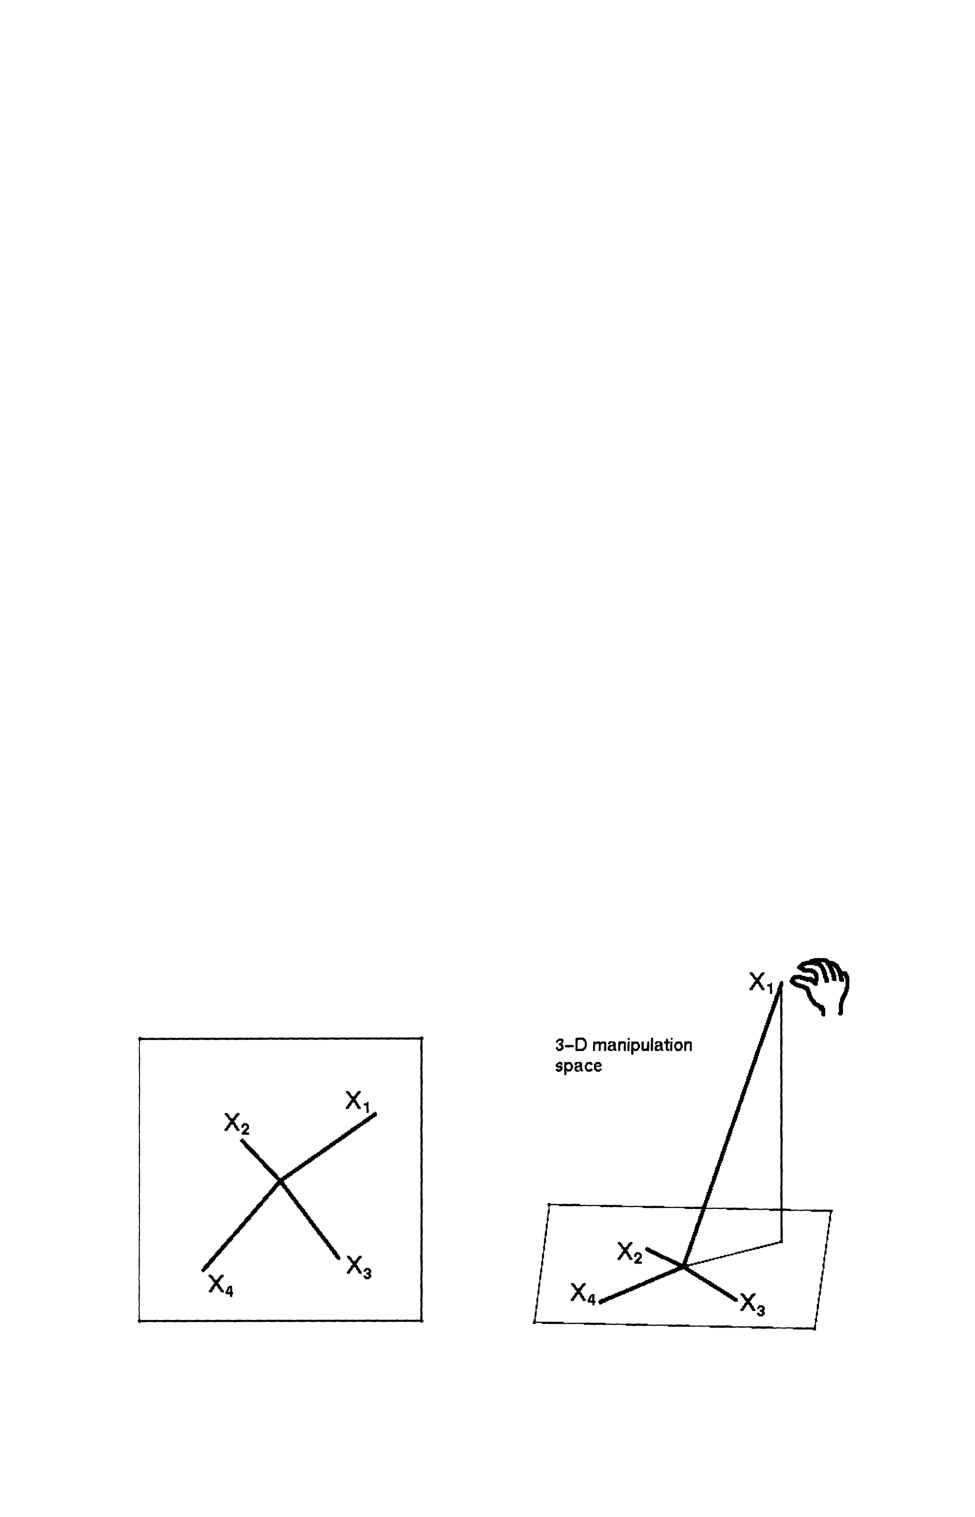
\includegraphics[width=0.8\textwidth]{figures/manip_space.pdf}}
\caption{Original contruction of the manual tour designed for 2D projections and created a 3D space from which to utilise track ball controls to change it's contribution. (Figure 3 from Cook and Buja (1997).)}
\label{manipspace}
\end{figure*}

\hypertarget{a-new-simpler-and-broadly-applicable-approach}{%
\subsection{A new simpler and broadly applicable
approach}\label{a-new-simpler-and-broadly-applicable-approach}}

The new approach emerged from experiments in mathematica. The components
corresponding to \(V_m\) are directly controlled by cursor movement,
which updates row \(m\) of \(A\). The updated matrix is then
orthonormalised.

\hypertarget{algorithm}{%
\subsubsection{Algorithm}\label{algorithm}}

\begin{enumerate}
\def\labelenumi{\arabic{enumi}.}
\item
  Provide \(A\), and \(m\). (Note that \(m\) could also be automatically
  chosen as the component that is closest to the cursor position.)
\item
  Change values in row \(m\), giving \(A^*\). A large change in these
  values would correspond to making a large jump from the current
  projection. Small changes would correspond to tracking a cursor,
  making small jumps from the current projection.
\item
  Orthonormalise \(A^*\), using Gram-Schmidt. For \(d=2\), and
  \(A^* = \left[ {\boldmath a}_{.1}~{\boldmath a}_{.2}\right]\), the
  steps are:

  \begin{enumerate}
  \def\labelenumii{\roman{enumii}.}
  \tightlist
  \item
    Normalise \({\boldmath a}_{.1}\), and \({\boldmath a}_{.2}\).
  \item
    \({\boldmath a}^*_{.2} = {\boldmath a}_{.2} - {\boldmath a}_{.1}^T{\boldmath a}_{.2}{\boldmath a}_{.1}\).
  \item
    Normalise \({\boldmath a}^*_{.2}\).
  \end{enumerate}
\end{enumerate}

This algorithm will produce the changes to a projection as illustrated
in Figure \ref{fig:manualsequence} (top row). The controlled variable,
\(V_m\), corresponds to the black line, and sequential changes to row
\(m\) of \(A\) can be seen to roughly follow a specified position
(orange dot). Changes in the other components happen as a result of the
orthonormalisation, but are uncontrolled.

\begin{figure}
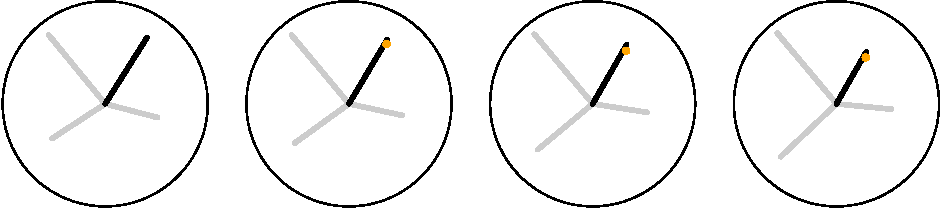
\includegraphics[width=1\linewidth]{paper_files/figure-latex/manualsequence-1} \caption{Sequence of projections where contribution of one variable is controlled (black) is changed: (top) unconstrained orthonormalisation, (bottom) constrained as specified. The dot (orange) indicates the chosen values for the controlled variable. For the constrained orthonormalisation it can be seen to precisely match the axis, but not so for the unconstrained orthonormalisation.}\label{fig:manualsequence}
\end{figure}

\hypertarget{refinements-to-enforce-exact-position}{%
\subsection{Refinements to enforce exact
position}\label{refinements-to-enforce-exact-position}}

The problem with new simple method (Algorithm 1) is that the precise
values for \(V_m\) cannot be specified because the orthonormalisation
will change them.

\hypertarget{adjustment-method-1}{%
\subsubsection{Adjustment method 1}\label{adjustment-method-1}}

A small modification to algorithm 1 will maintain the components of
\(V_m\) precisely (Figure \ref{fig:manualsequence} (bottom row)). It is
as follows:

\begin{enumerate}
\def\labelenumi{\arabic{enumi}.}
\tightlist
\item
  Provide \(A\), and \(m\).
\item
  Change values in row \(m\), giving \(A^*\).
\item
  Store row \(m\) separately, and zero the values of row \(m\) in
  \(A^*\), giving \(A^{*0}\).
\item
  Orthonormalise \(A^{*0}\), using Gram-Schmidt.
\item
  Replace row \(m\) with the original values, giving \(A^{**}\).
\item
  For \(d=2\), adjust the values of \({\boldmath a}^{**}_{.2}\) using
\end{enumerate}

\[a^{**}_{j2}+\frac{a_{m1}a_{m2}}{p-1}, j=1, ..., p, j\neq m\].

which ensures that

\[\sum_{j=1, j\neq m}^p a^{**}_{j1}a^{**}_{j2} + a_{m1}a_{m2} = 0\].

If \(d>2\) the process would be sequentially repeated in the same manner
that Gram-Schmidt is applied sequentially to orthormalise the columns of
a matrix. If \(d=1\) no orthonormalisation is needed, and the projection
vector would simply need to be normalized after each adjustment.

\hypertarget{adjustment-method-2}{%
\subsubsection{Adjustment method 2}\label{adjustment-method-2}}

For \(d=2\) projections, the projection matrix is the sub-matrix of
\(A\) formed by its first two columns. Whereas orthonormality of the
basis for the p-dimensional space is given by
\(e_i\cdot e_j=\delta_{ij},{i,j,=1,\cdots,}\), orthonormality of the
projection matrix is expressed as
\(P_i\cdot P_j=\delta_{ij}, {i,j=1,2}\). Movement of the cursor takes
the two components \({x_{m1},x_{m2}}\) into a selected new value
\({a,b}\). Although the motion is constrained by \(a^2+b^2\leq 1\), this
is not sufficient to guarantee orthonormality of the new projection
matrix. One possible algorithm to achieve this is

\begin{enumerate}
\item Cursor movement takes ${x_{m1},x_{m2}}\to {a,b}$
\item The freedom to change the components $A_{i3}\cdots A_{ip}$ (the columns of $A$ not corresponding to the projection matrix) is used to select a new orthonormal basis as follows:
\begin{enumerate}
\item For row $m$ one chooses $A_{m3}=\sqrt{1-a^2-b^2},~A_{m,k>3}=0$
\item For other rows, $A_{i\neq m,j\geq3}$ random selections in the range $(-1,1)$ are made.
\item The Gram-Schmidt algorithm is then used to obtain an orthonormal basis taking $e_m$ as the first vector (which is already normalized), and then proceeding as usual $e_1\to e_1-(e_1\cdot e_m) e_m$, $e_1\to e_1/(e_1\cdot e_1)$, etc.
\end{enumerate}
\item this results in the orthonormal basis $A^*$ and a new projection matrix with $P_{m1}=a,~P_{m2}=b$.
\end{enumerate}

The random choice for the components of \(A\) not in the projection
matrix allows the exploration of dimensions perpendicular to the
projection plane.

\begin{align}
A=~~~& \begin{pNiceArray}{ccccc}[first-row,first-col]
\CodeBefore
       \columncolor{red!15}{1,2}
              \rowcolor{blue!15}{4}
     \Body
       & \stackrel{P_1}{\downarrow} & \stackrel{P_2}{\downarrow} &  & &\\
e_1\to & x_{11} & x_{12}  & x_{13} & \cdots & x_{1p} \\
e_2 \to& x_{21}  & x_{22}  & \cdot  &\cdots & x_{2p} \\
\vdots ~~~&\vdots & \vdots  & \vdots & \ddots & \vdots \\ 
 e_m \to& x_{m1}  & x_{m2}  & \cdot  &\cdots & x_{mp} \\   
\vdots ~~~&\vdots & \vdots  & \vdots & \ddots & \vdots \\
e_p \to&x_{p1} & x_{p2} &\cdot &\cdots & x_{pp} 
\end{pNiceArray},\quad (x_{m1},x_{m2})\to (a,b)
\end{align}

\hypertarget{adjustment-method-3}{%
\subsubsection{Adjustment method 3}\label{adjustment-method-3}}

For now just sketching the idea:

\begin{itemize}
\tightlist
\item
  first step is to click on the axis display to change the contribution
  of one variable \(m\)
\item
  capture that position and replace the corresponding row in the
  projection matrix
\item
  for 2D projection this gives components \(m_1\) along ``x'' direction
  and \(m_2\) along \(y\) direction
\item
  next step: rotate basis such that direction of row m now corresponds
  to the first basis vector, this means we apply 2x2 rotation matrix to
  each row of the projection matrix, where the rotation angle is
  \(tan(\theta) = m_2/m_1\) (that matrix can be written just in terms of
  that ratio, \(x= m_2/m_1\), when \(m_1<0\) I think we just need to
  translate \(\theta \rightarrow \theta + \pi\))
\item
  take the rotated basis, apply Gram-Schmidt, now the direction of \(m\)
  will not change (but the length will change during normalization)
\item
  rotated back to the original xy basis to update the plots
\end{itemize}

XXX need to check calculation of angle when \(m_1 < 0\)

\hypertarget{sec:implementation}{%
\section{Experimenting with new techniques using
Mathematica}\label{sec:implementation}}

\begin{itemize}
\tightlist
\item
  \textbf{Why is this a good sandbox}
\item
  \textbf{Explain the functionality available in the notebooks}
\end{itemize}

The following functions are implemented in the Mathematica package
\texttt{mmtour.wl}:

\begin{itemize}
\item
  \texttt{ProjectionPlot{[}data,\ projmat,\ xRange(=Automatic),\ yRange(=Automatic),\ \ colour(=Automatic){]}}
  with arguments

  \begin{itemize}
  \tightlist
  \item
    \texttt{data}: A list of data matrices (they must all have the same
    dimensionality)
  \item
    `\texttt{projmat}: A projection matrix which describes the
    projection plane. This is the initial projection and does not need
    to be orthonormal (XXX is this right?).
  \item
    `\texttt{xRange}: A list which details the range of the horizontal
    axis.
  \item
    `\texttt{yRange}: A list which details the range of the vertical
    axis.
  \item
    `\texttt{colour}: A list of graphics directives to be applied to
    each data matrix.
  \end{itemize}
\end{itemize}

There are problems with the default values for x and y ranges and
colour. It would be better to fix the ranges and colour based on the
data as well as the origin of axes and the size of the points.

\textbf{It would be good if the initial projection matrix (and maybe the
center) had default values. Perhaps a random matrix with the correct
dimensions read from the data? Fix 1}

The format for the printed projection matrix can be improved also. Maybe
fix the number of digits and the position of the label.

\begin{itemize}
\item
  \texttt{SlicePlot{[}data,\ projmat,\ centrePoint,\ height,\ heightRange,\ ptSize1(=0.005),\ ptSize2(=0.004),\ minDist(=0){]}}
  with arguments (used to be called SliceDynamic in Alex's first
  version, the name SliceDynamic was taken by something else below)

  \begin{itemize}
  \tightlist
  \item
    \texttt{data}: A data matrix
  \item
    \texttt{projmat}: The inital projection matrix
  \item
    \texttt{centrepoint}: The initial position of the slice
  \item
    \texttt{height}: The initial height of the slice
  \item
    \texttt{heightRange}: The range of heights
  \item
    \texttt{ptSize1}: The size of the points that exist within the slice
  \item
    \texttt{ptSize2}: The size of the points that exist outside of the
    slice
  \end{itemize}
\end{itemize}

This function requires some auxiliary functions. It does not accept more
than one data set.

\textbf{It would be good if the initial projection matrix (and maybe the
center) had default values. Perhaps a random matrix with the correct
dimensions read from the data?}

It may be good to fix the size of the points, the center of the axes and
the scales of the axes rather than allow them to change as the
projection and slicing changes

\begin{itemize}
\item
  \texttt{SliceDynamic{[}data,\ projmat,\ centrePoint,\ height,\ heightRange,\ ptSize1\ :\ 0.005,\ ptSize2\ :\ 0.004{]}}
  with arguments
\item
  \texttt{data}: A data matrix with an extra grouping or clustering
  column (numerical)
\item
  \texttt{projmat}: The initial projection matrix
\item
  \texttt{centrepoint}: The initial position of the slice
\item
  \texttt{height}: The initial height of the slice
\item
  \texttt{heightRange}: The range of heights
\item
  \texttt{ptSize1}: The size of the points that exist within the slice
\item
  \texttt{ptSize2}: The size of the points that exist outside of the
  slice
\end{itemize}

\textbf{Does this need to be a separate function from SlicePlot? Fix 2}

\textbf{It would be good if the initial projection matrix (and maybe the
center) had default values. Perhaps a random matrix with the correct
dimensions read from the data? Fix 3}

\textbf{It may be good to fix the size of the points, the center of the
axes and the scales of the axes rather than allow them to change as the
projection and slicing changes. Fix 4}

\textbf{I have found it useful to input different data sets rather than
have this function sort them automatically using the last column. One
data set with a flag column at the end, is best! Is the code too
complicated? Fix 5}

\begin{itemize}
\tightlist
\item
  \texttt{Projected2DSliderPlot{[}{]}}
\end{itemize}

This function uses a different display for the projection that I find
very useful. However as it stands it is specific to one data set. Needs
to be generalised to arbitrary data if we want to keep it.

\textbf{For Alex to do}

\begin{itemize}
\tightlist
\item
  \textbf{We would need a screenshot (and video) for each of these.}
\item
  \textbf{Fix 1, 2, 3, 4, 5}
\item
  \textbf{Code consistent for applications to work - see
  slice\_tour\_compare\_sets.nb. See below}

  \begin{itemize}
  \tightlist
  \item
    \textbf{We need to make sure the drawing range is fixed (no resizing
    of the axis when changing projection or slicing). It could be nice
    if there was a manual zoom in/zoom out to change scale
    occasionally.}
  \item
    \textbf{Should also make sure the size of the points is fixed (maybe
    this will be automatic if the drawing range is fixed?), bigger
    points would be preferred, currently the size is sometimes really
    tiny and it becomes difficult to see anything.}
  \item
    \textbf{Can we have some heuristic to decide the range for the slice
    thickness slider? In the second graph there is a tiny part of the
    slider where the changes are interesting, difficult to navigate
    since this makes it super sensitive to any small movement, while
    most of the options are not interesting. My suggestion would be to
    keep (as I understand is the case now) the maximum thickness (all
    points in) as the upper bound, but instead of zero use a thickness
    below which slices tend to be empty as the lower bound.}
  \item
    \textbf{For the olives example I think the relation between x2 and
    the blue region could be interesting.}
  \item
    \textbf{pdfsense data: can we use random samples instead of the
    first 10k rows? Then we should still be able to see the bigger
    picture (with picking the first ones we get some artificial
    structure from how the data was sampled initially).}
  \item
    \textbf{I was playing around with this today. Looks like the axes
    are fixed when changing slice thickness, but not when rotating?}
  \item
    \textbf{Anyways, some observations that might be useful, but all of
    this seems difficult for including in a paper:}
  \item
    \textbf{In the first example we can show how the yellow group is
    associated with the first variable (x1, I guess this is C9?) - when
    slicing through the center it only appears when x1 has a bigger
    component on the projection, it is associated with low values of x1.
    Since they are not near the average value of x1 the points do not
    get captured in a slice where x1 is not important in the projection.
    We can move the center point to -1 in the first component to then
    explore how the yellow group relates to the other three variables.
    Much less clear, maybe some indication of smaller x2 and larger x3
    for this.}
  \item
    \textbf{The second example is too busy for manual exploration I
    would say (too many axes to move around separately).}
  \item
    \textbf{Third example could be similar to the first: blue region
    requires small values of x2, can be understood from the exploration,
    then move center point to -0.5 in x2 to explore further. Now
    interpretation becomes tricky. Sometimes blue and yellow seem just
    randomly everywhere, sometimes blue more contained in an ellipsoid
    around the center (indicating some correlation between variables).
    For example try zeroing out components 2 and 3 to see this slice in
    x1 vs x4.}
  \item
    \textbf{For the last example x4 seems to be the one to work with. I
    feel like this is again very similar, maybe better to instead
    explore other examples (maybe something without slicing?)}
  \end{itemize}
\end{itemize}

\begin{figure}

{\centering 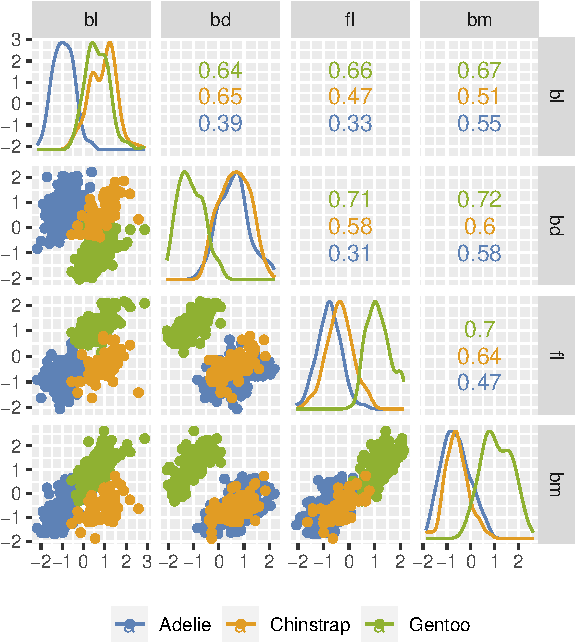
\includegraphics[width=0.8\linewidth]{paper_files/figure-latex/penguins-scatmat-1} 

}

\caption{Scatterplot matrix of the (standardised) penguins data. The three species are reasonably different in size, with Gentoo distinguised from the other two on body depth relative to flipper length and body mass.}\label{fig:penguins-scatmat}
\end{figure}

\hypertarget{sec:examples}{%
\section{Application}\label{sec:examples}}

To illustrate the usefulness of the manual controls we use the 4D
penguins data \citep{penguins}. We will show how classification
boundaries can be explored and better understood on projections and
slices through 4D space. Figure \ref{fig:penguins-scatmat} shows a
scatterplot matrix of this data. There are four variables
(\texttt{bl\ =\ bill\_length\_mm,\ bd\ =\ bill\_depth\_mm,\ fl\ =\ flipper\_length\_mm,\ bm\ =\ body\_mass\_g})
measuring the size of the penguins from three species (Adelie, Chinstrap
and Gentoo). The scatterplot matrix shows that the three species appear
to be likely separable, and that at least the Gentoo can be
distinguished from the other two species when \texttt{bd} is paired with
\texttt{fl} or \texttt{bm}. The steps for exploring boundaries in this
example are as follows:

\begin{enumerate}
\def\labelenumi{\arabic{enumi}.}
\tightlist
\item
  Build your classification model.
\item
  Predict the class for a dense grid of values covering the data space.
\item
  Examine projections, using a manual tour so that the contribution of
  any variable is controlled.
\item
  Slice through the center, to explore where the boundaries will likely
  meet.
\item
  Move the slice by changing the center in the direction of a single
  variable to explore the extent of a boundary for a single group
  relative to a variable.
\end{enumerate}

\hypertarget{constructing-the-4d-prediction-regions}{%
\subsection{Constructing the 4D prediction
regions}\label{constructing-the-4d-prediction-regions}}

We use the \texttt{classifly} package \citep{classifly} to generate
predictions across the 4D cube spanned by the data, with two
classification models: linear discriminant analysis (LDA) and random
forest (RF).

\hypertarget{exploring-projections-manually}{%
\subsection{Exploring projections
manually}\label{exploring-projections-manually}}

We start by first exploring the projections of the model prediction.
Figure \ref{proj1} summarises the process. Through manual rotation of
the view we can get a feeling for where in the space we primarily
predict each of the three species, and we also get a sense of the
difference between the two models. To illustrate this difference we have
manually rotated the projection for the RF model (left plot) to identify
a projection that shows the non-linear but block-type structure that is
typical of this type of model. This particular projection (\(A_1\)) is
exported so that the same projection can be used to show the LDA model
(middle plot) and the actual data (right plot). What can be seen is the
linearity of the LDA model, where the boundaries are linear and oblique
to the variable axes. And, interestingly this particular projection of
the original data shows very distinct clusters of the three species.
That means, the obscuring of the boundaries between groups for both of
the models is driven by what is happening in the orthogonal space to the
plane of the selected projection.

\begin{figure*}[ht]
\centerline{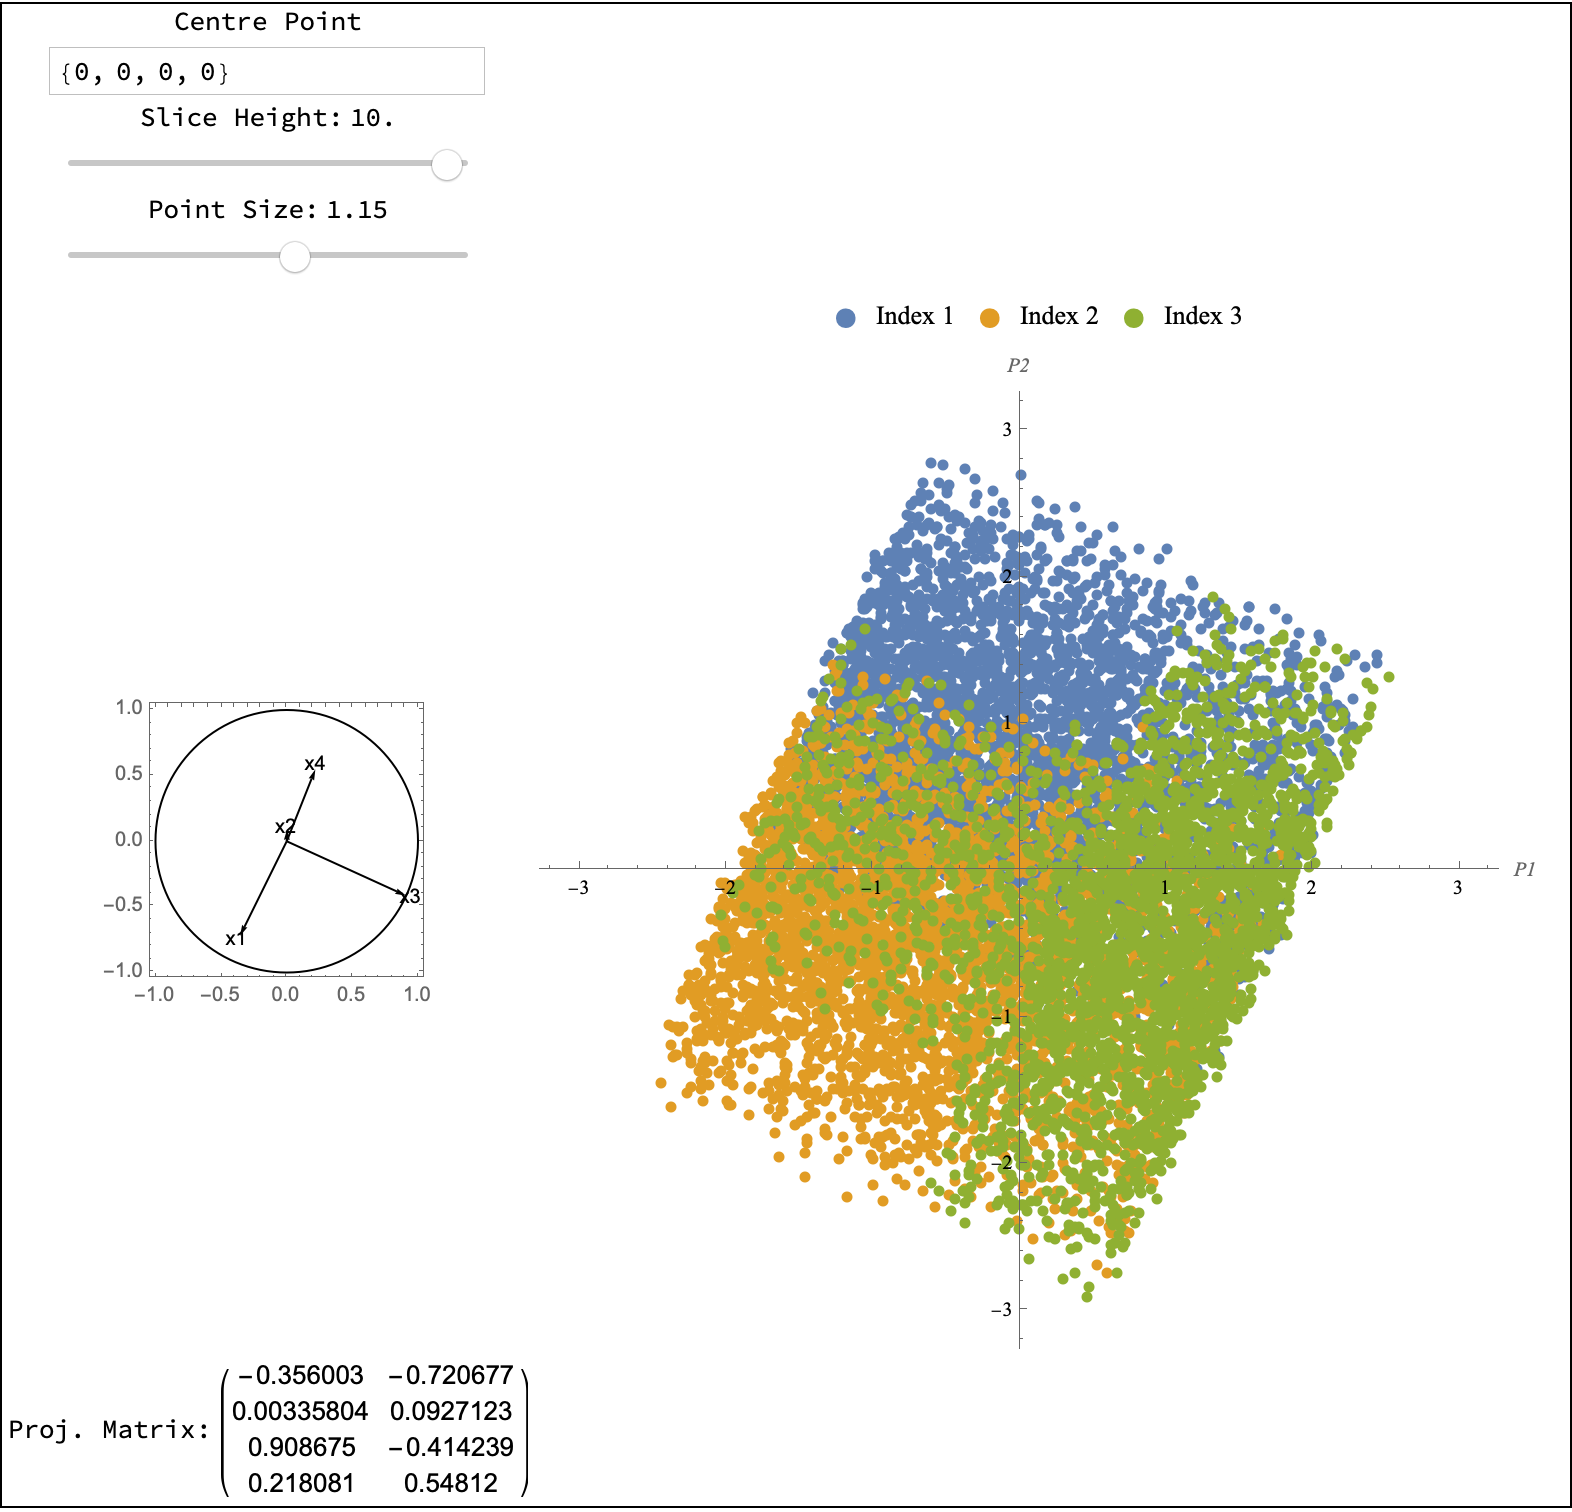
\includegraphics[width=0.32\textwidth]{figures/proj1_rf.png}
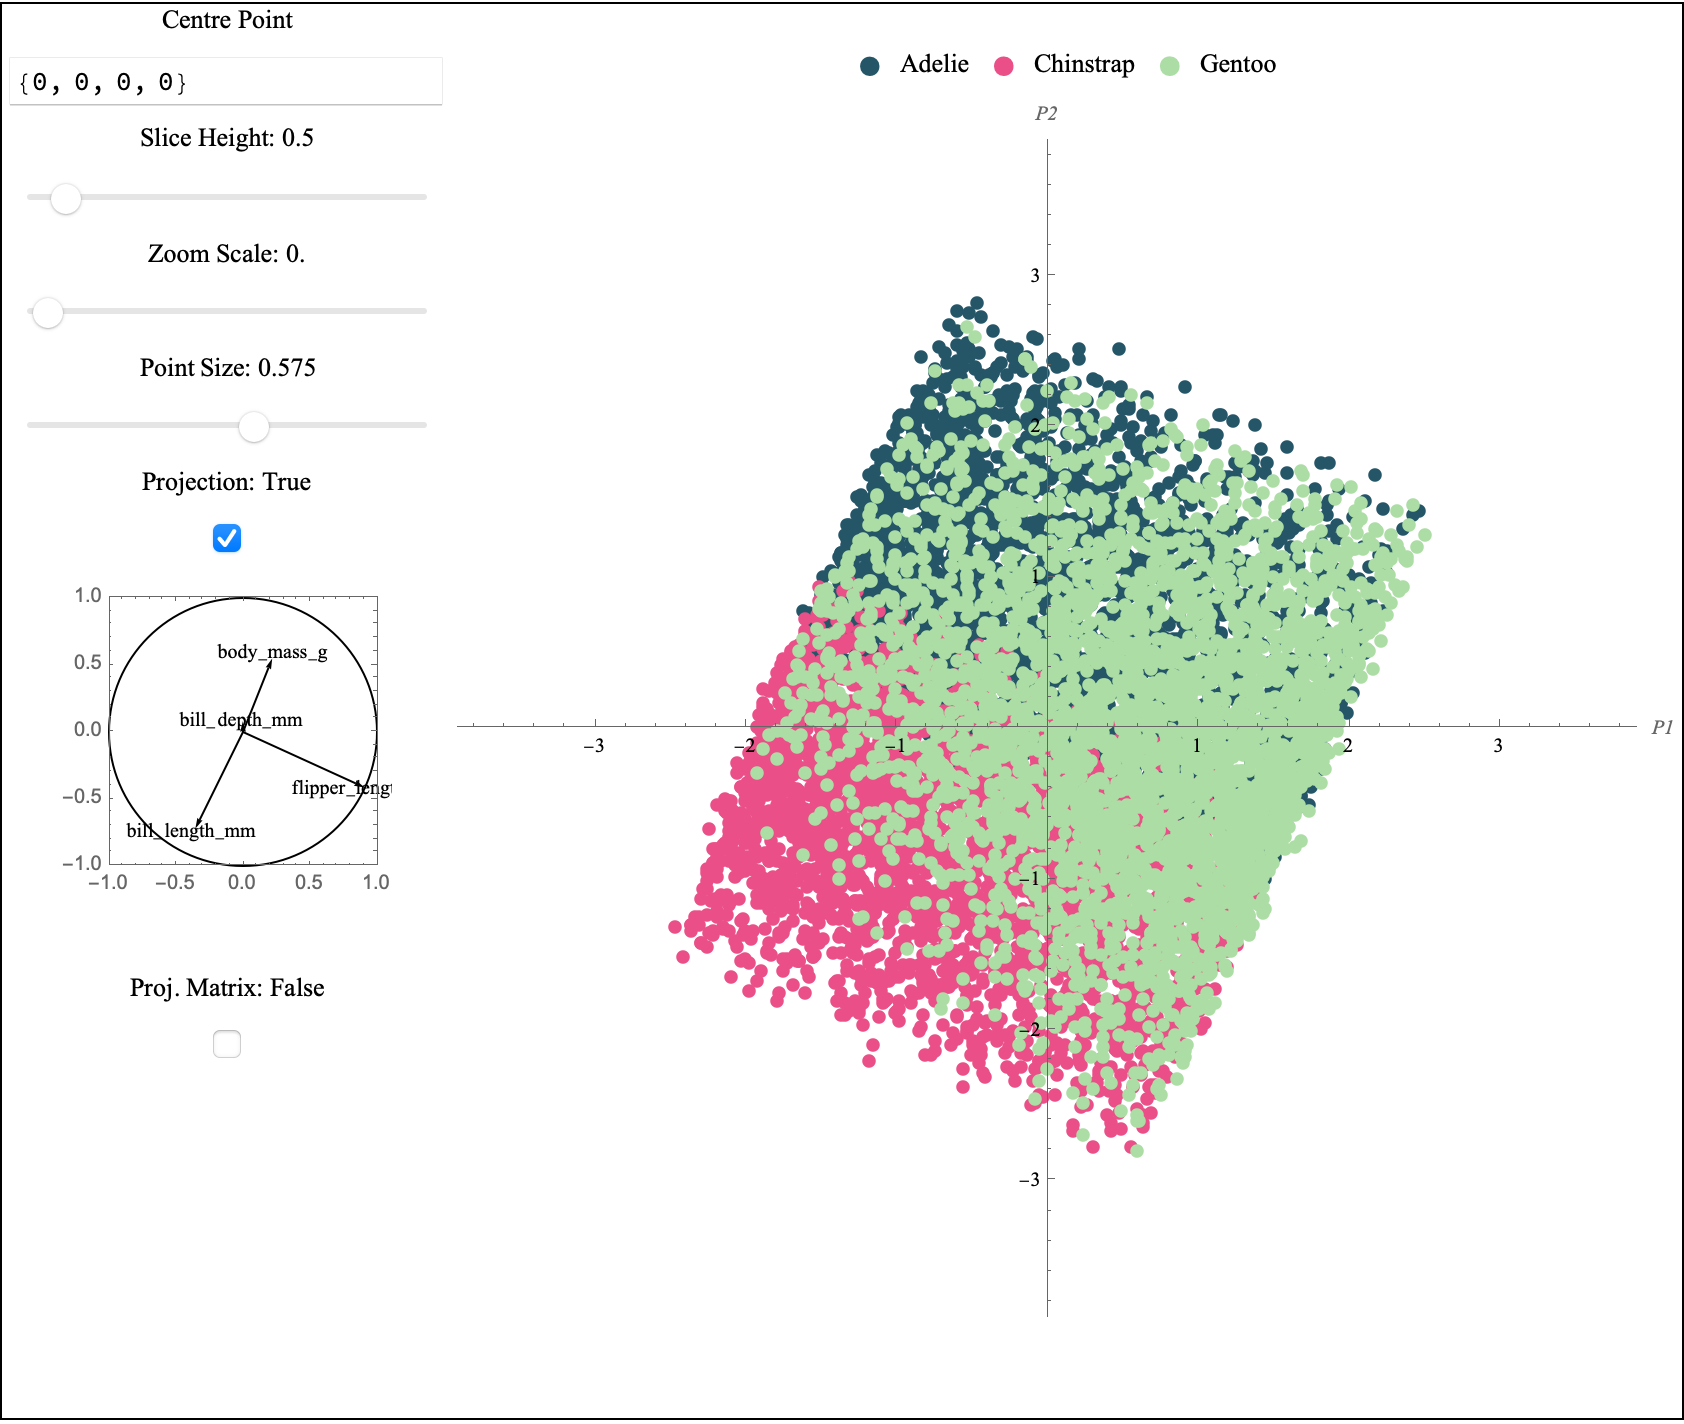
\includegraphics[width=0.32\textwidth]{figures/proj1_lda.png}
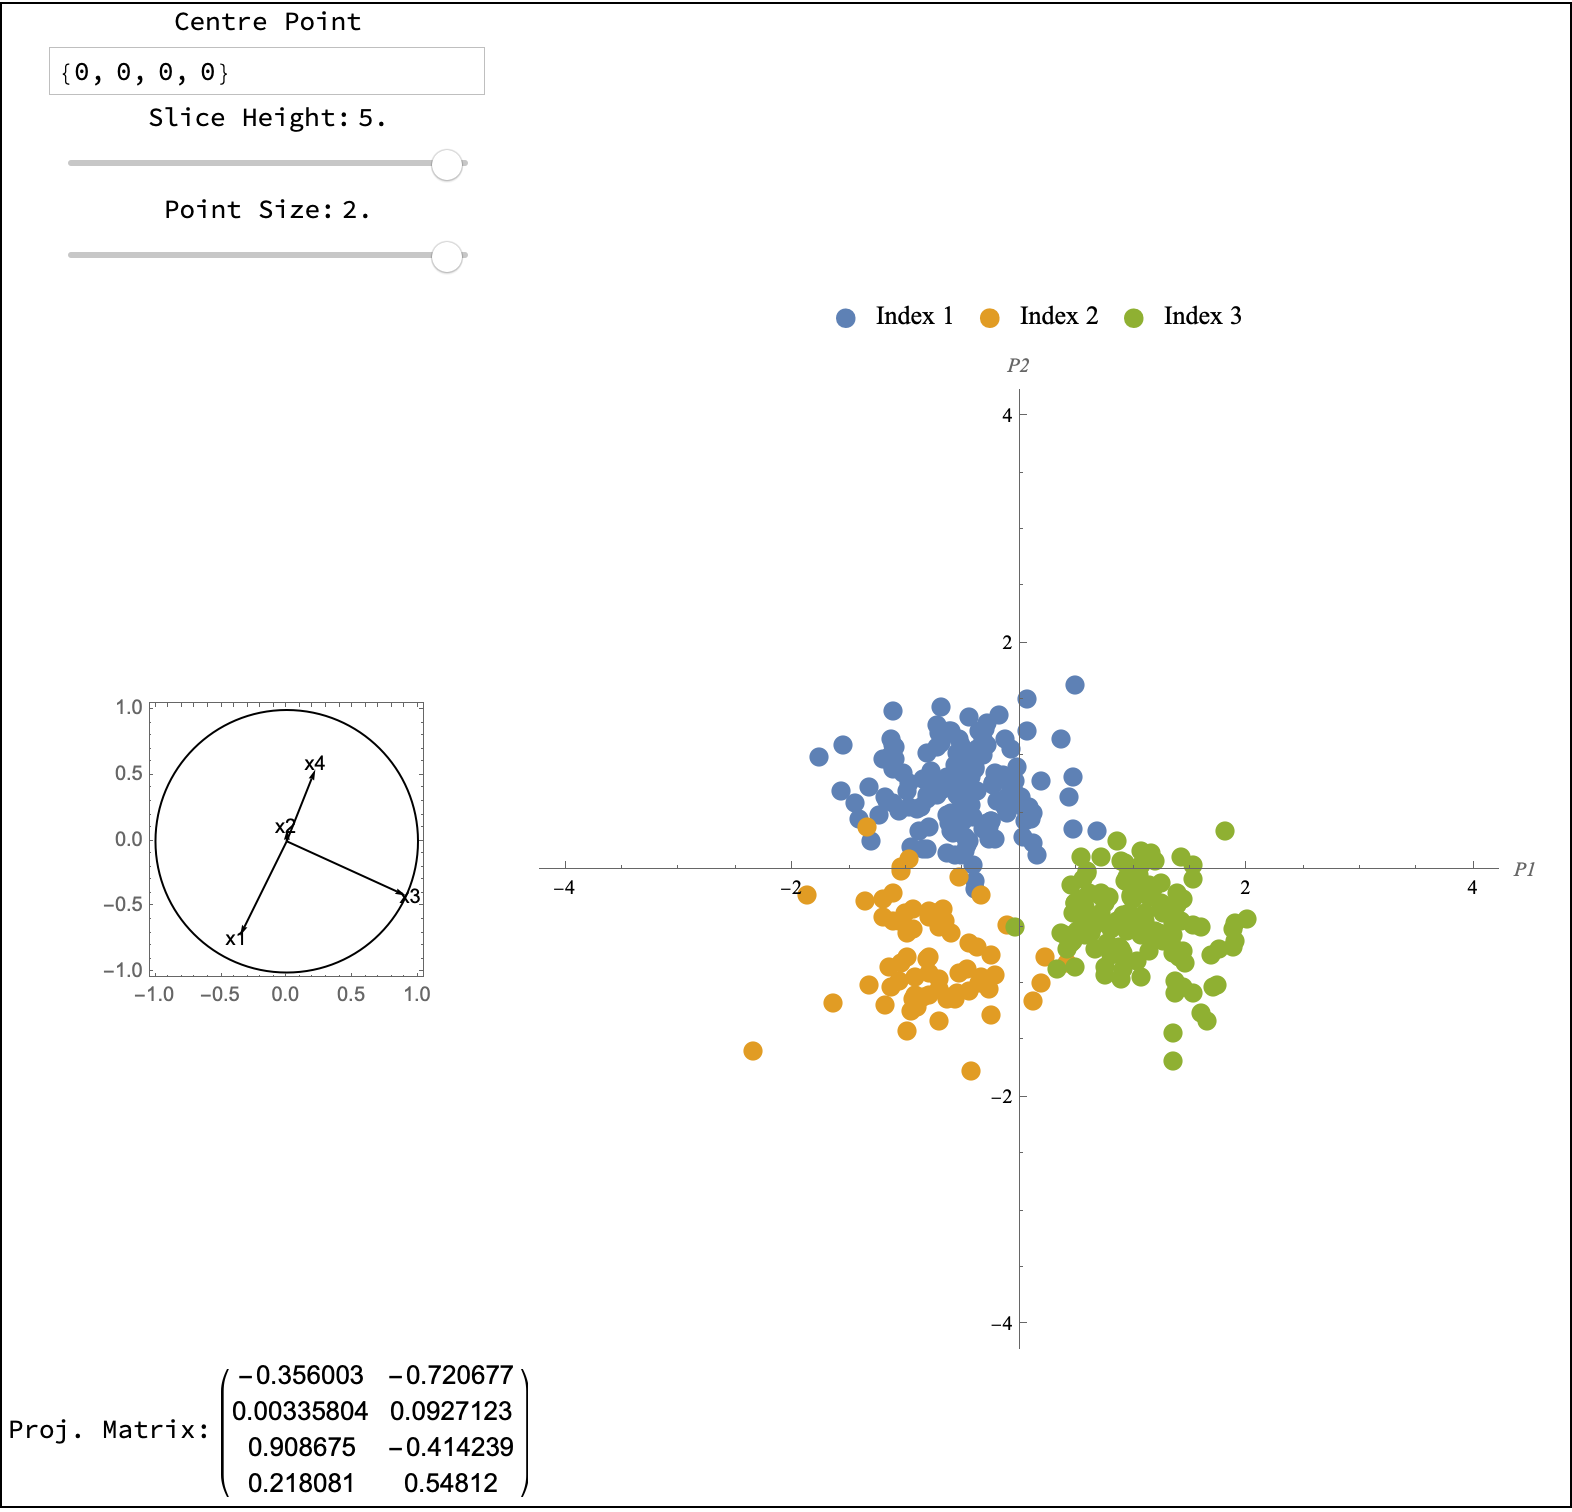
\includegraphics[width=0.32\textwidth]{figures/proj1_data.png}}
\caption{Projection identified using the manual tour, because it reveals an interesting structure in the predictions from the RF model (left). We can clearly see a block structure, while the LDA model (middle) produces linear boundaries. The three groups are nicely separated in this projection of the data (right)}.
\label{proj1}
\end{figure*}

\hypertarget{slicing-through-the-center}{%
\subsection{Slicing through the
center}\label{slicing-through-the-center}}

XXXX currently in the notebook \(A_1\) is called A5, and \(A_2\) is
called A6

We continue the investigation by now slicing based on the projection
\(A_1\). For both models we look at a thin (\(h=0.5\)) slice through the
center, \(S_1^0\). As a first option we explore how manually changing
the projection away from \(A_1\) can help with understanding the
boundary better. For our example we notice that \(A_1\) does not contain
any contribution from the second variable (\texttt{bd}), and in our
illustration we will first rotate this variable into the view.

We again start by looking at the RF model, the slice \(S_1^0\) shows the
block structure of the model, with the third group (green, Gentoo
penguins) overlapping with both of the other groups (Fig. \ref{slice1},
top-left). This is similar for the LDA model (Fig. \ref{slice1},
top-right), but again the linearity results in different boundaries and
thus differences in how the classes overlap.

By rotating in the second variable we can find a view that shows three
neatly separated blocks for the RF model, and we export the
corresponding projection matrix \(A_2\) to see the same views for the
LDA model which also shows a neater separation of the classes along the
boundary (see bottom row of Fig. \ref{slice1}).

Finally we look at the data projection based on \(A_2\) and find that
the third group (green, Gentoo penguins) is further away from the other
two groups (compared to \(A_1\)), see Fig. \ref{proj2}.

\begin{figure*}[ht]
\centerline{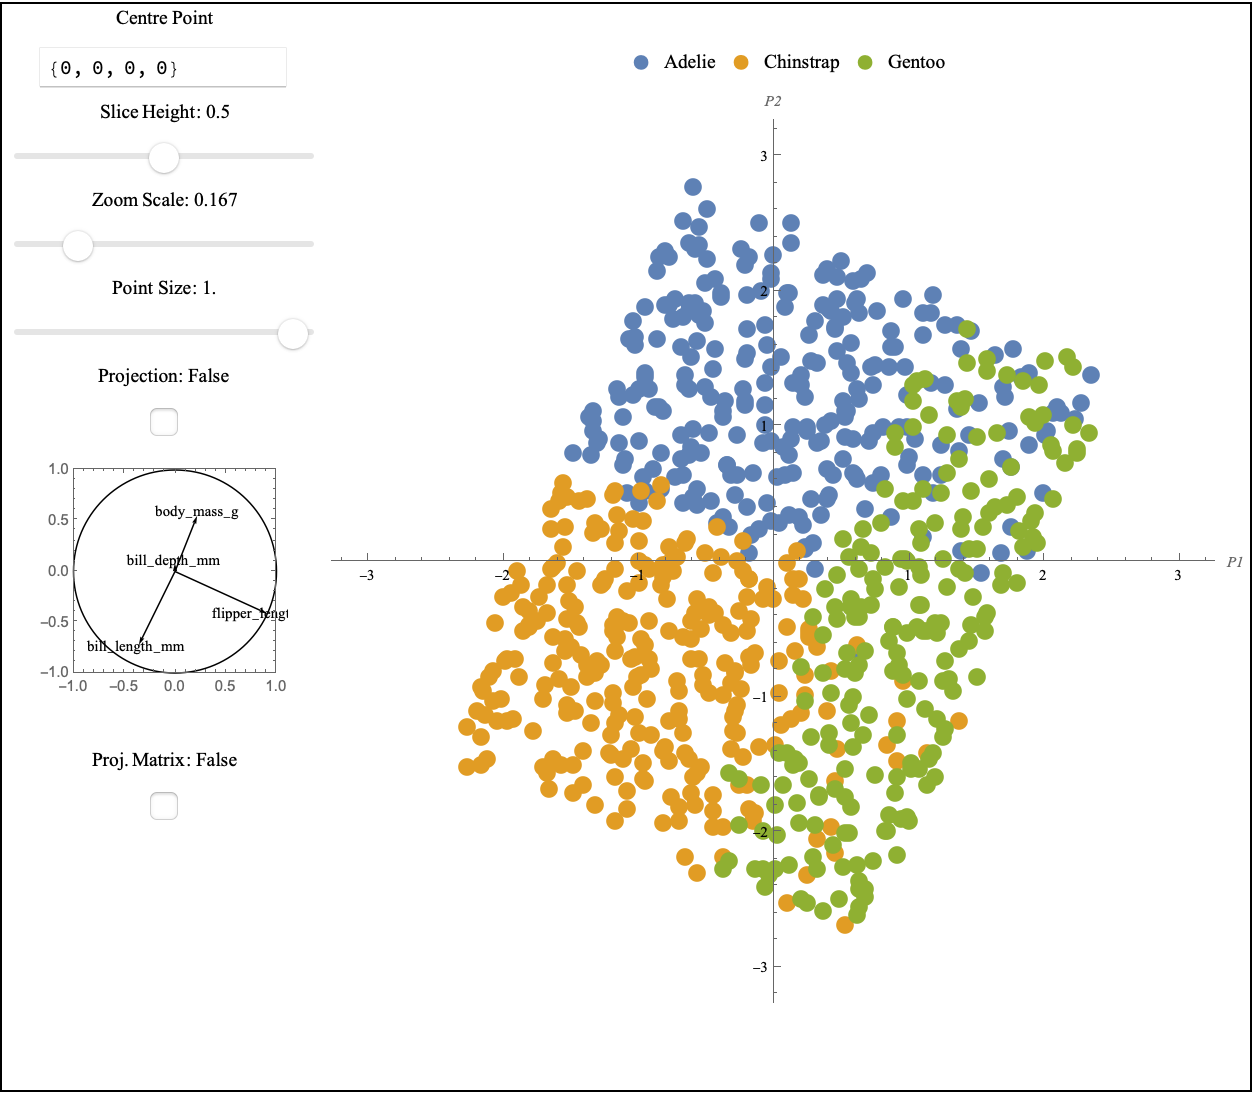
\includegraphics[width=0.45\textwidth]{figures/slice1_rf.png}
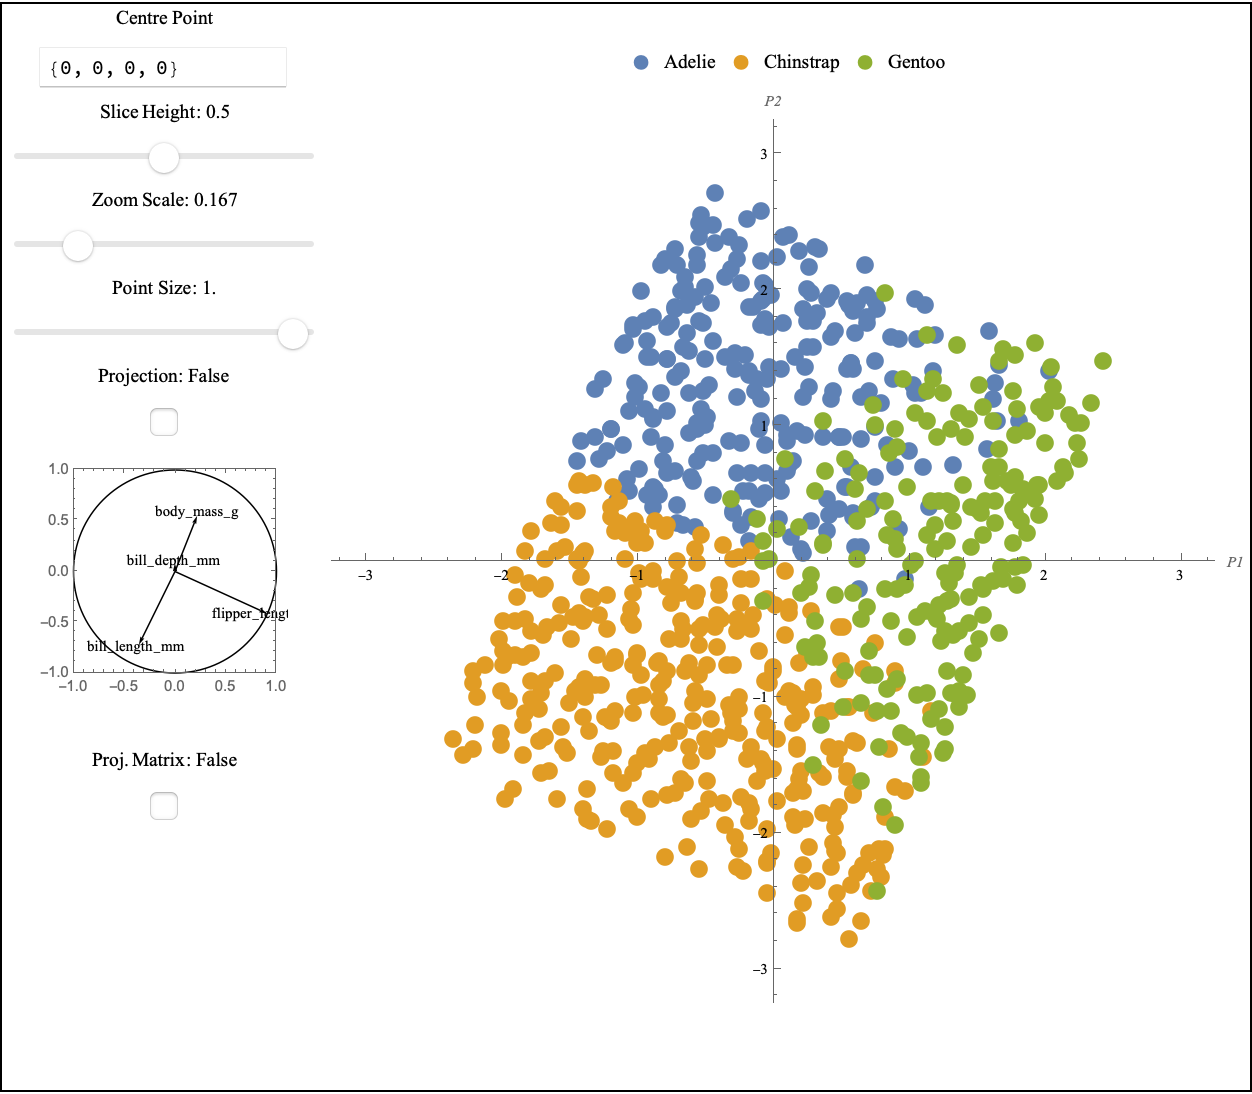
\includegraphics[width=0.45\textwidth]{figures/slice1_lda.png}}
\centerline{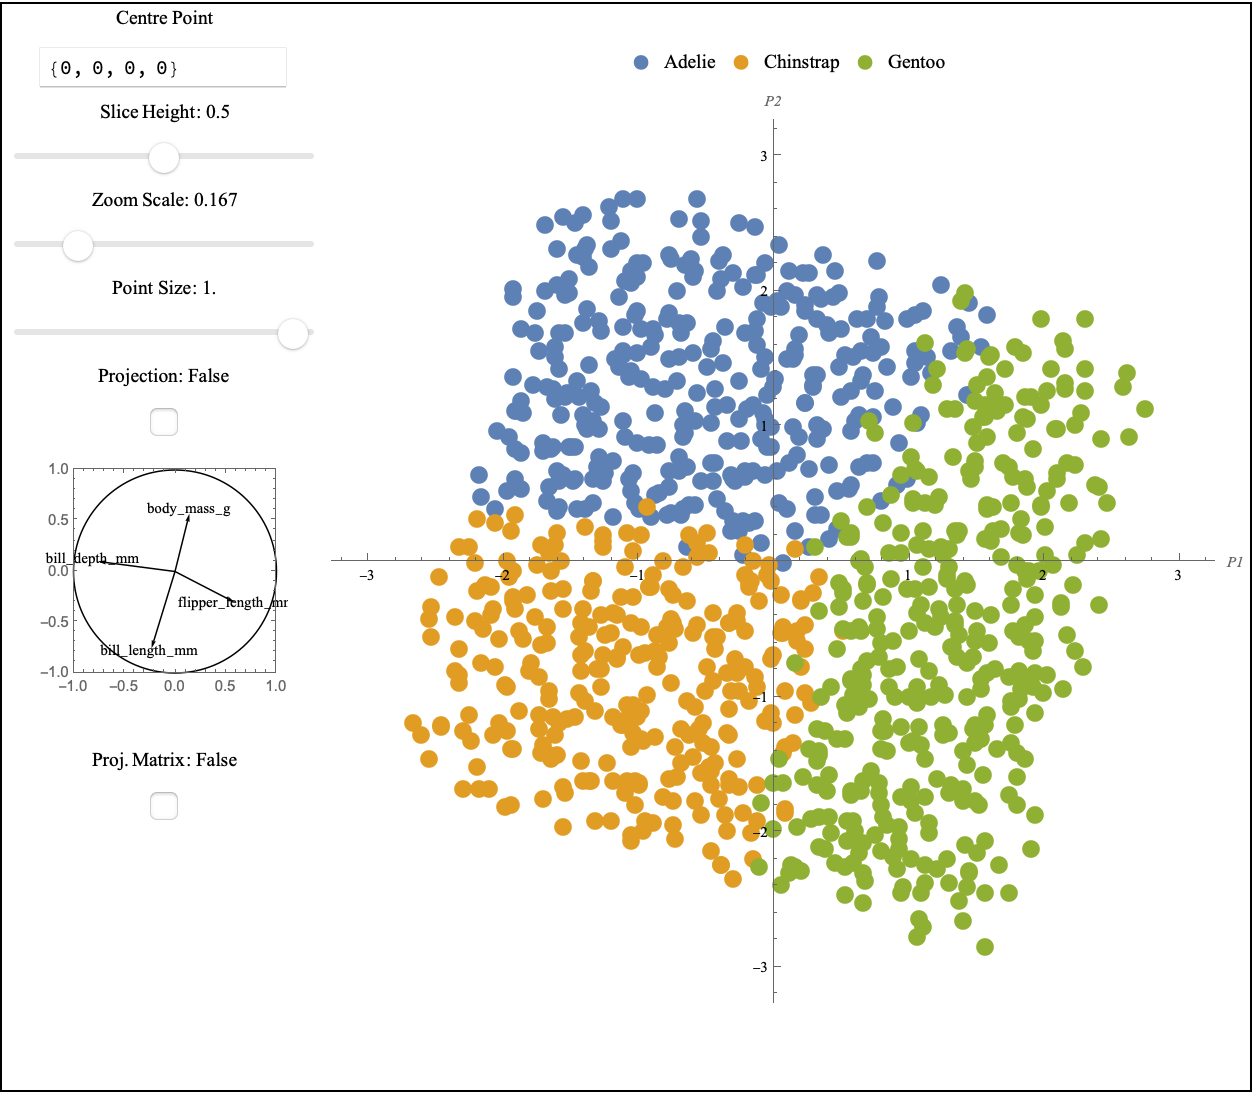
\includegraphics[width=0.45\textwidth]{figures/slice2_rf.png}
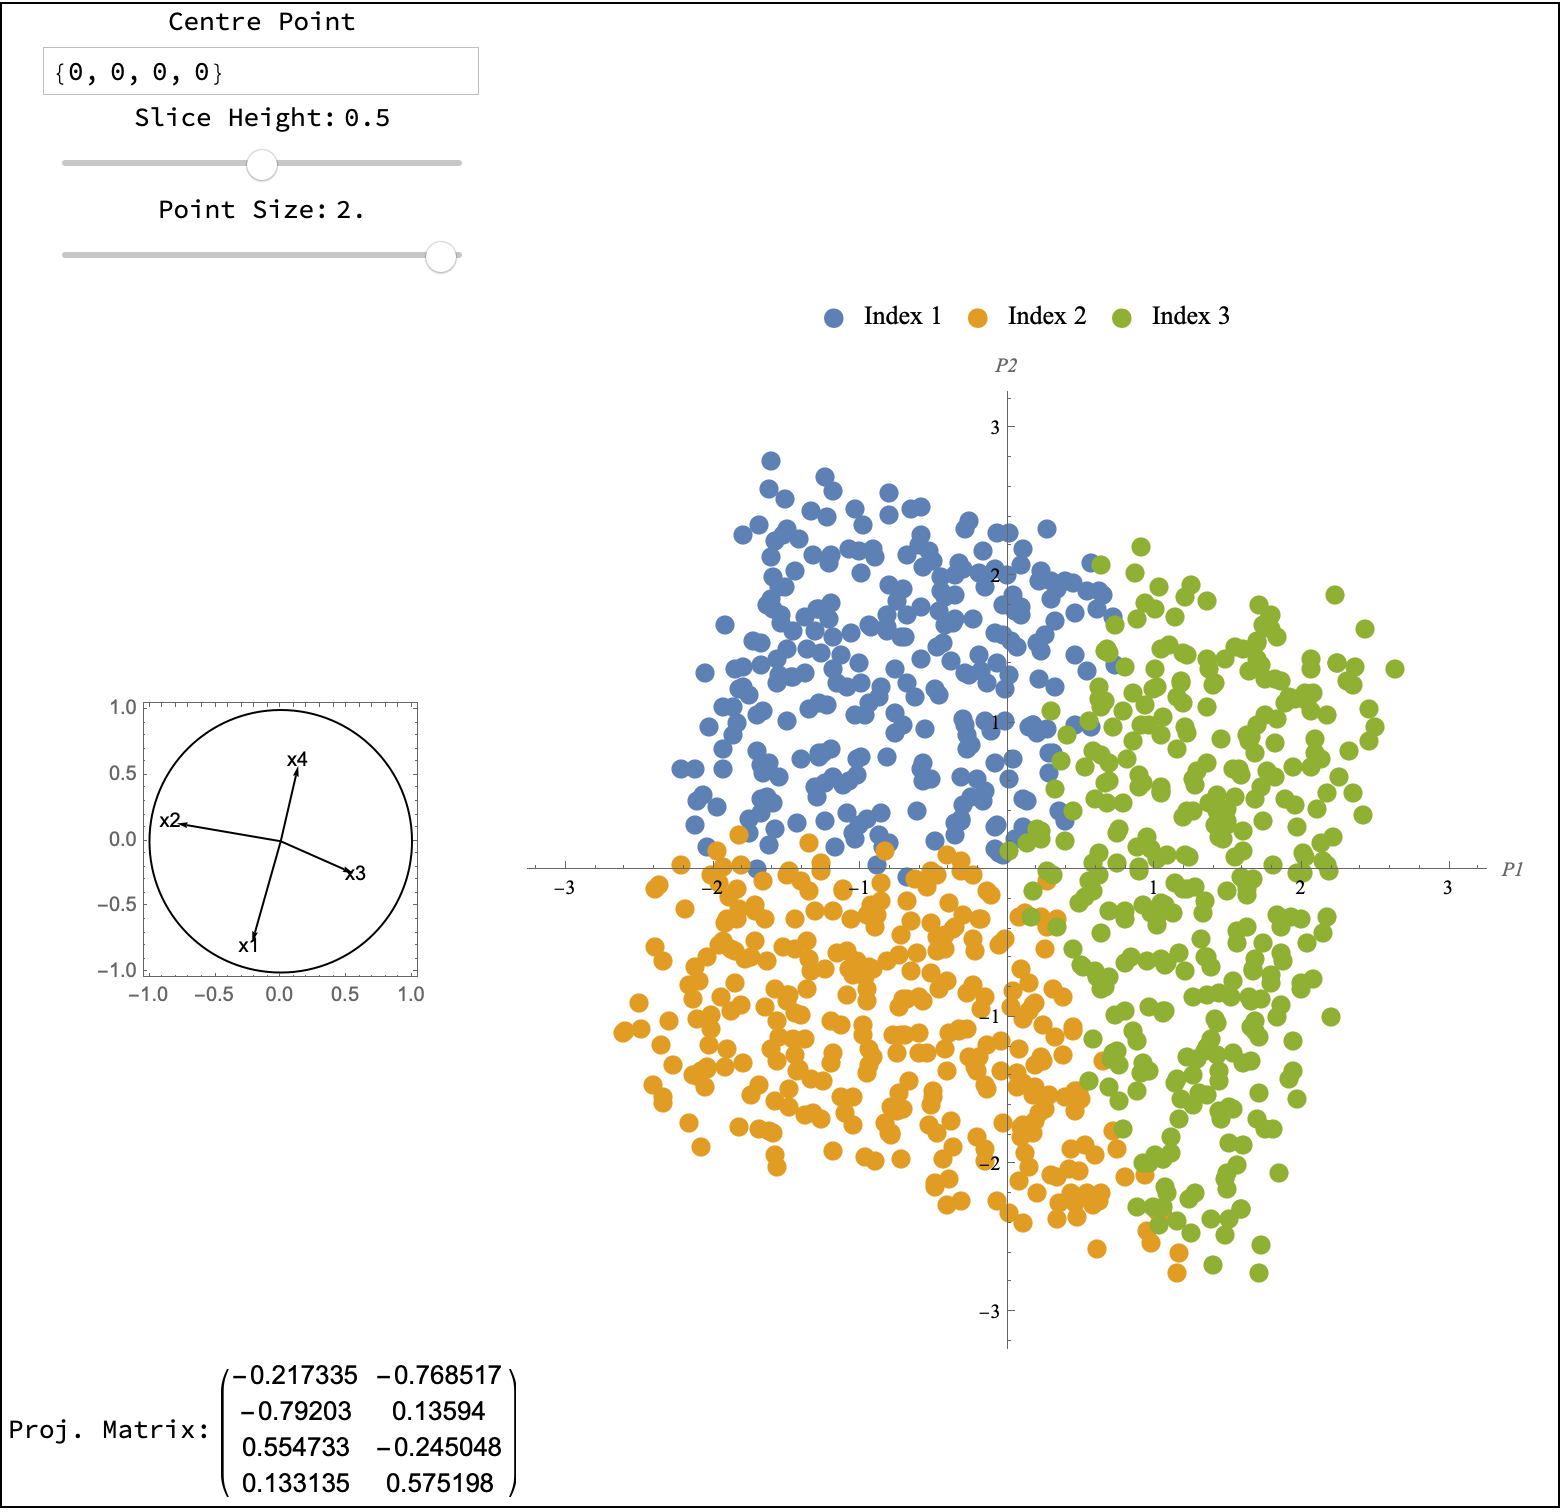
\includegraphics[width=0.45\textwidth]{figures/slice2_lda.png}}
\caption{Comparing slices based on two projections $A_1$ (top row) and $A_2$ (bottom row), for the two models RF (left) and LDA (right). With $A_1$ we see two groups overlap (green - Gentoo with yellow - Chinstrap), while the rotation to $A_2$ results in clear boundaries inside the slice. The boundary between Adelie (blue) and Chinstrap (yellow) is similar for both models but very different between Chinstrap and Gentoo (green).}
\label{slice1}
\end{figure*}

\begin{figure*}[ht]
\centerline{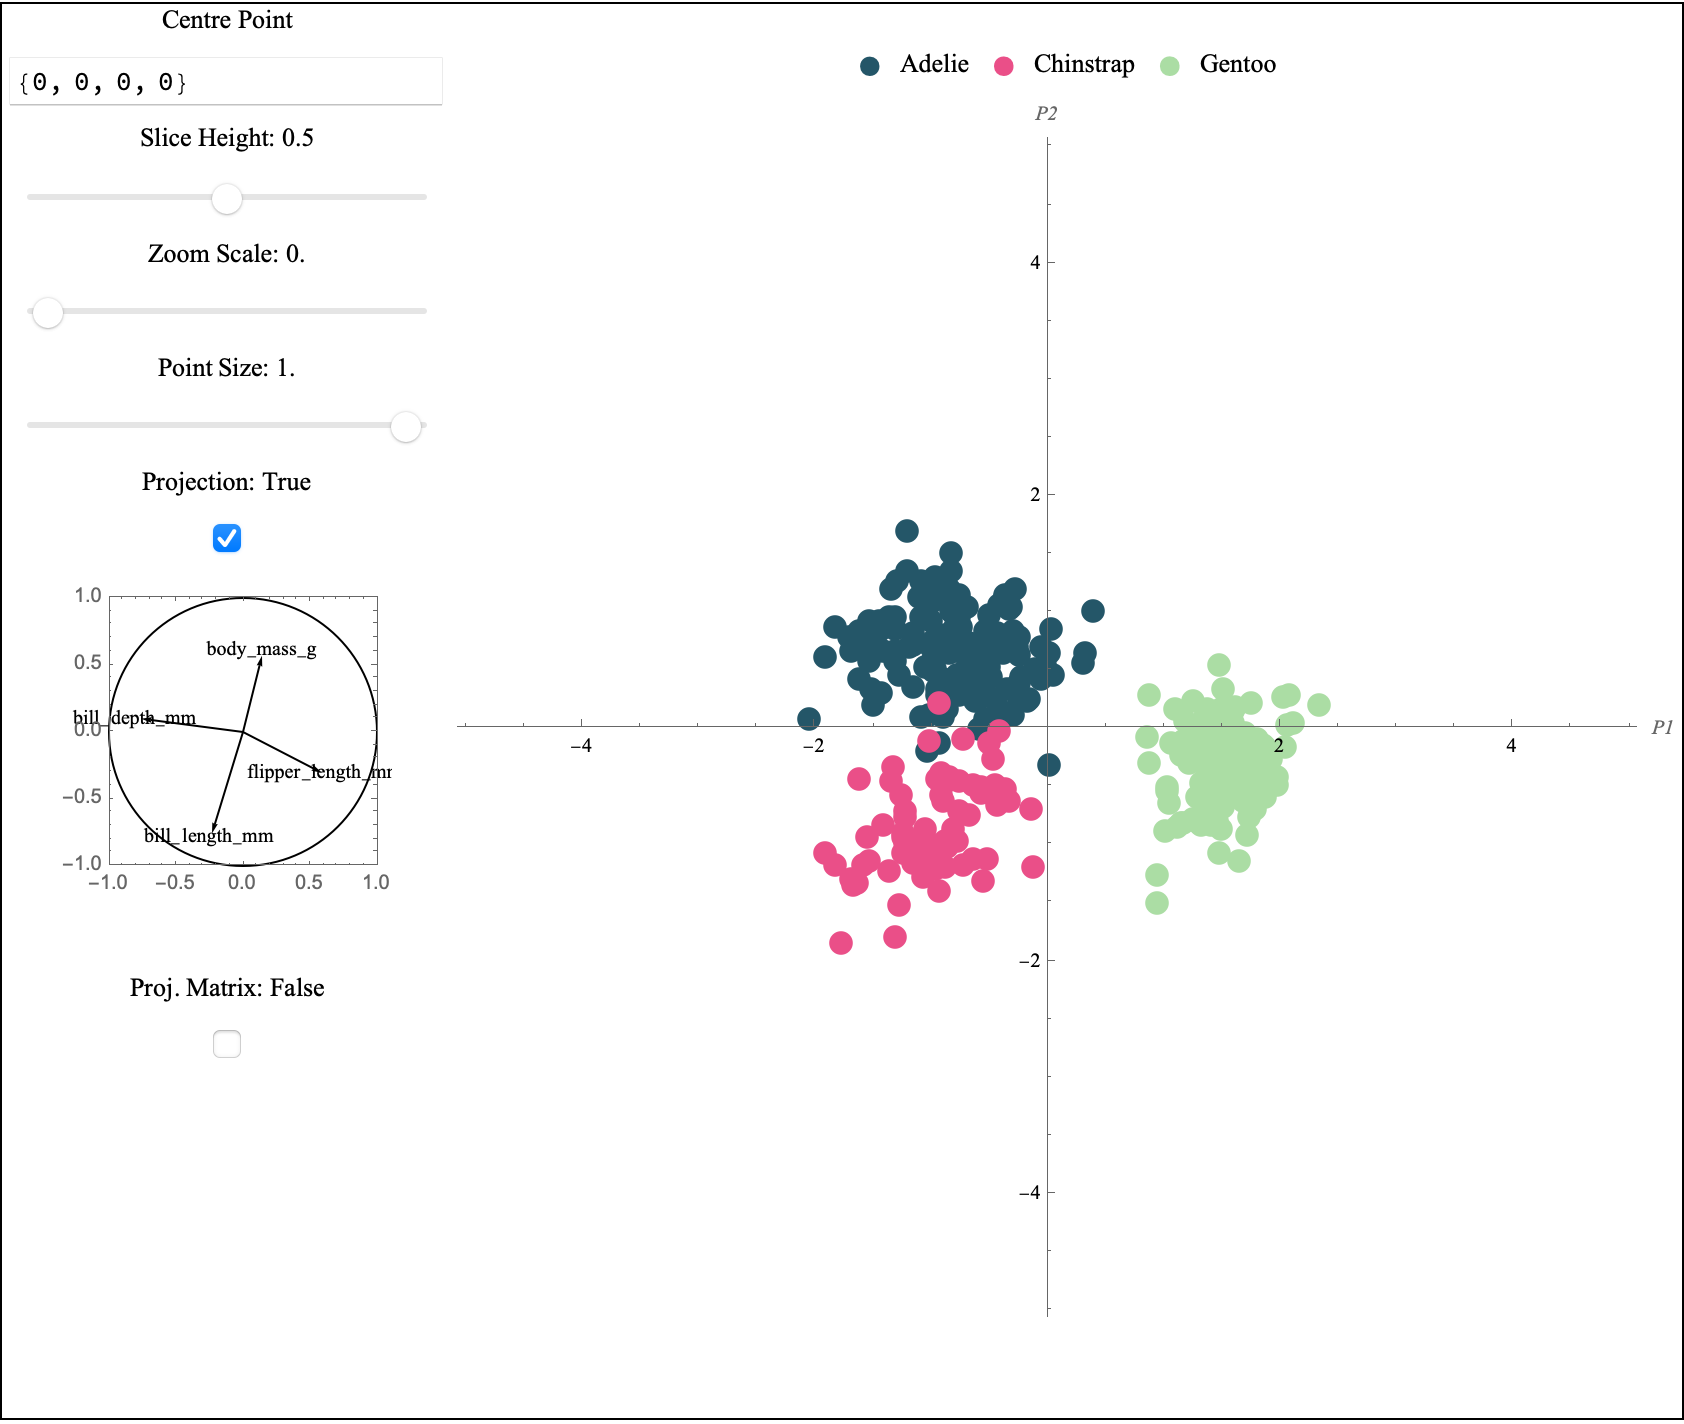
\includegraphics[width=0.45\textwidth]{figures/proj2_data.png}}
\caption{Projection of the data based on $A_2$. Compared to projecting onto $A_1$ we see that the green observations (Gentoo) are more separated from the other two species.}
\label{proj2}
\end{figure*}

\hypertarget{shifting-the-slice-center}{%
\subsection{Shifting the slice center}\label{shifting-the-slice-center}}

We have seen that starting from \(A_1\) using the manual controls to
change the contribution of the second variable we could find a clear
separation boundary indicating the relation between this variable (bill
depth) and the Gentoo penguin species. Instead of rotating to a
different projection, we might also change the view by moving the slice
along one direction in the 4D space. Here we will continue our
exploration of the dependence on \texttt{bd} and move the slice defined
by \(A_1\) to either large or small values of the bill depth
(\(\pm 1.5\) after centering and scaling). We will label these slices as
\(S_1^{\pm}\). Here we will also look at slices of the observed data
points, using a thicker slice (\(h=1.5\)) to capture enough points in a
given view.

We start by a comparison of the two models and the data distribution in
\(S_1^{+}\), thus the slice is localized towards high values of bill
depth in Fig. \ref{slice1p}. We can see that all three slices (the two
models and the data) contain almost no points from the third class
(green, Gentoo), and that the decision boundary between the two models
is very similar.

\begin{figure*}[ht]
\centerline{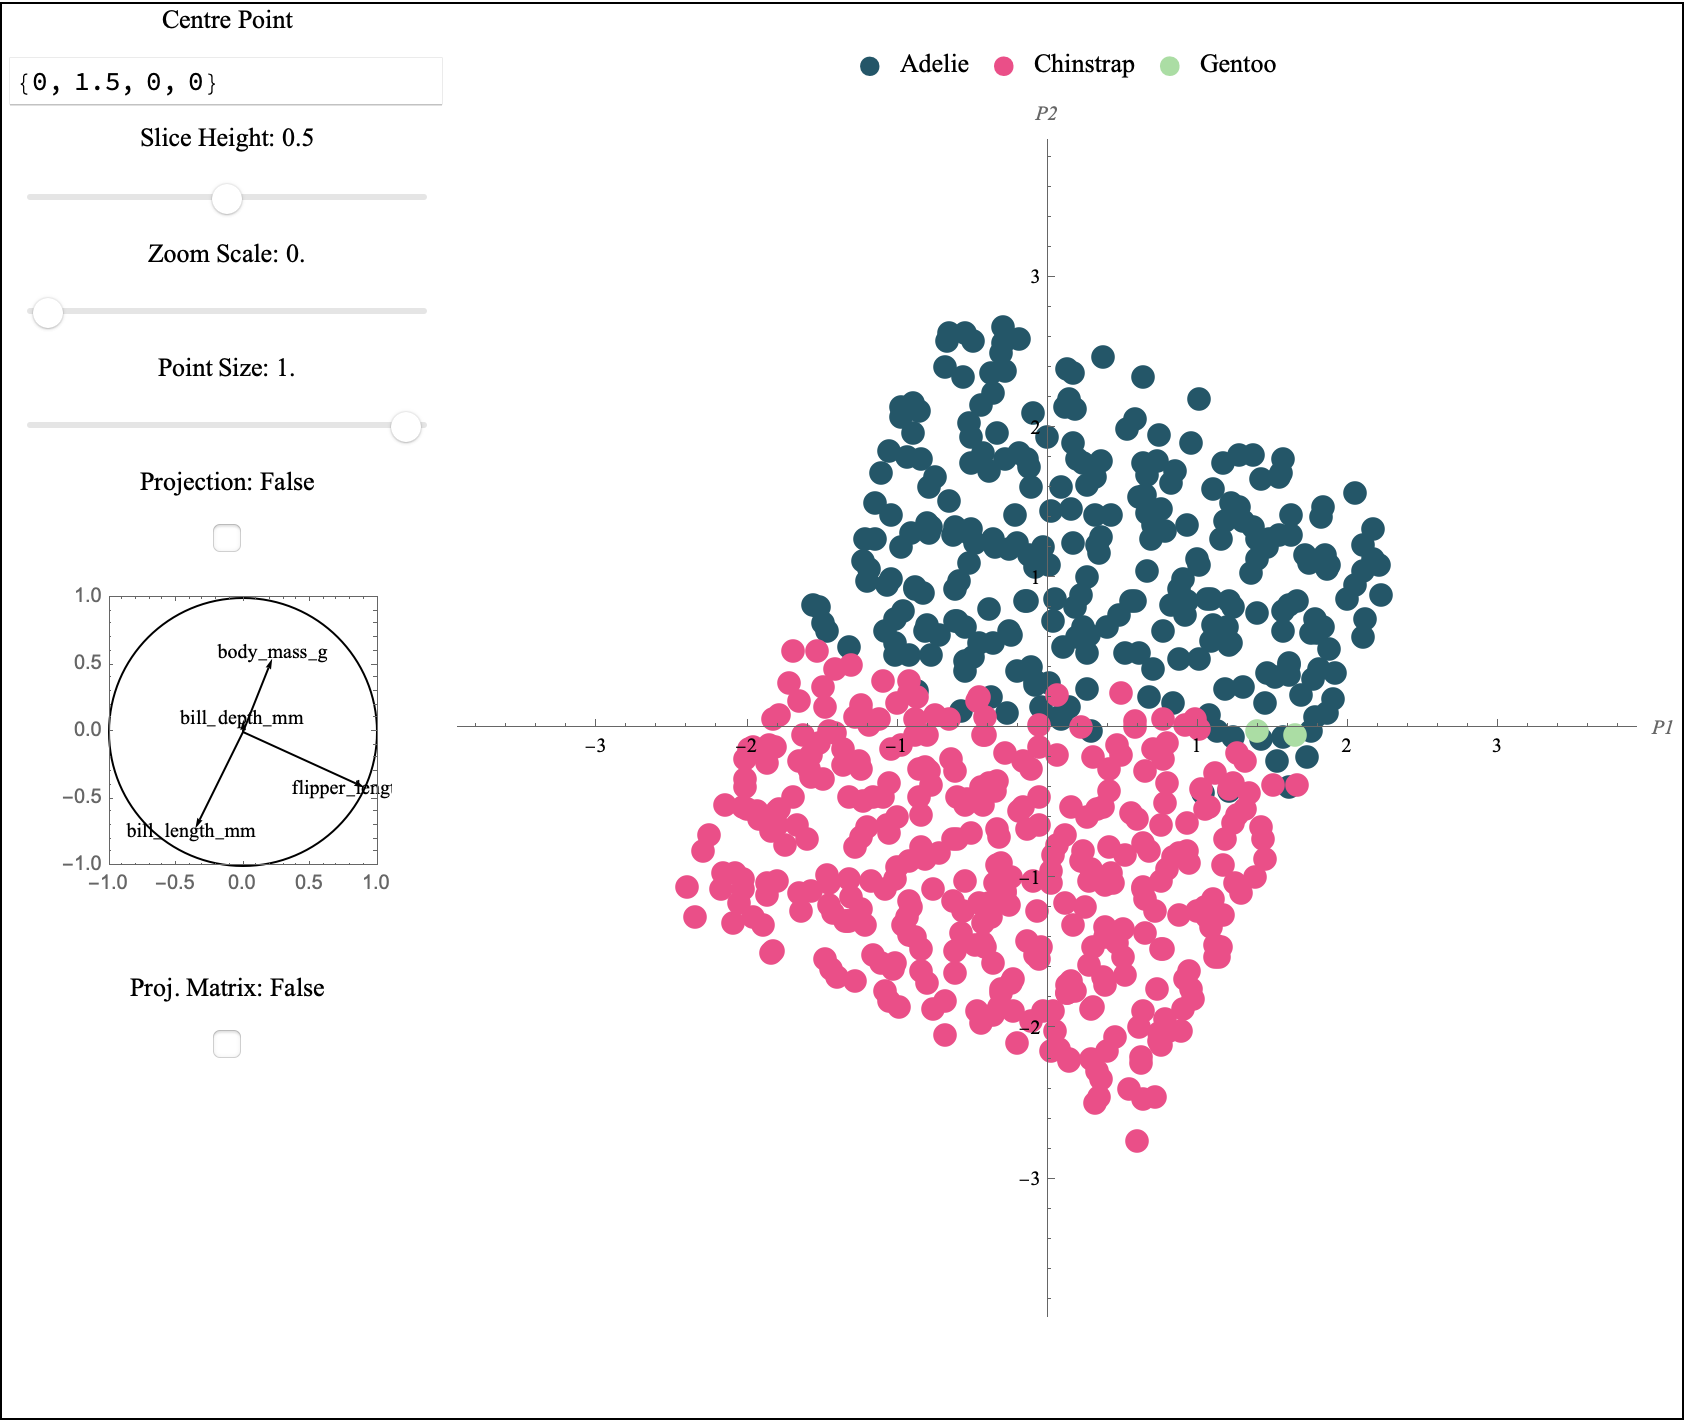
\includegraphics[width=0.32\textwidth]{figures/slice1_p_rf.png}
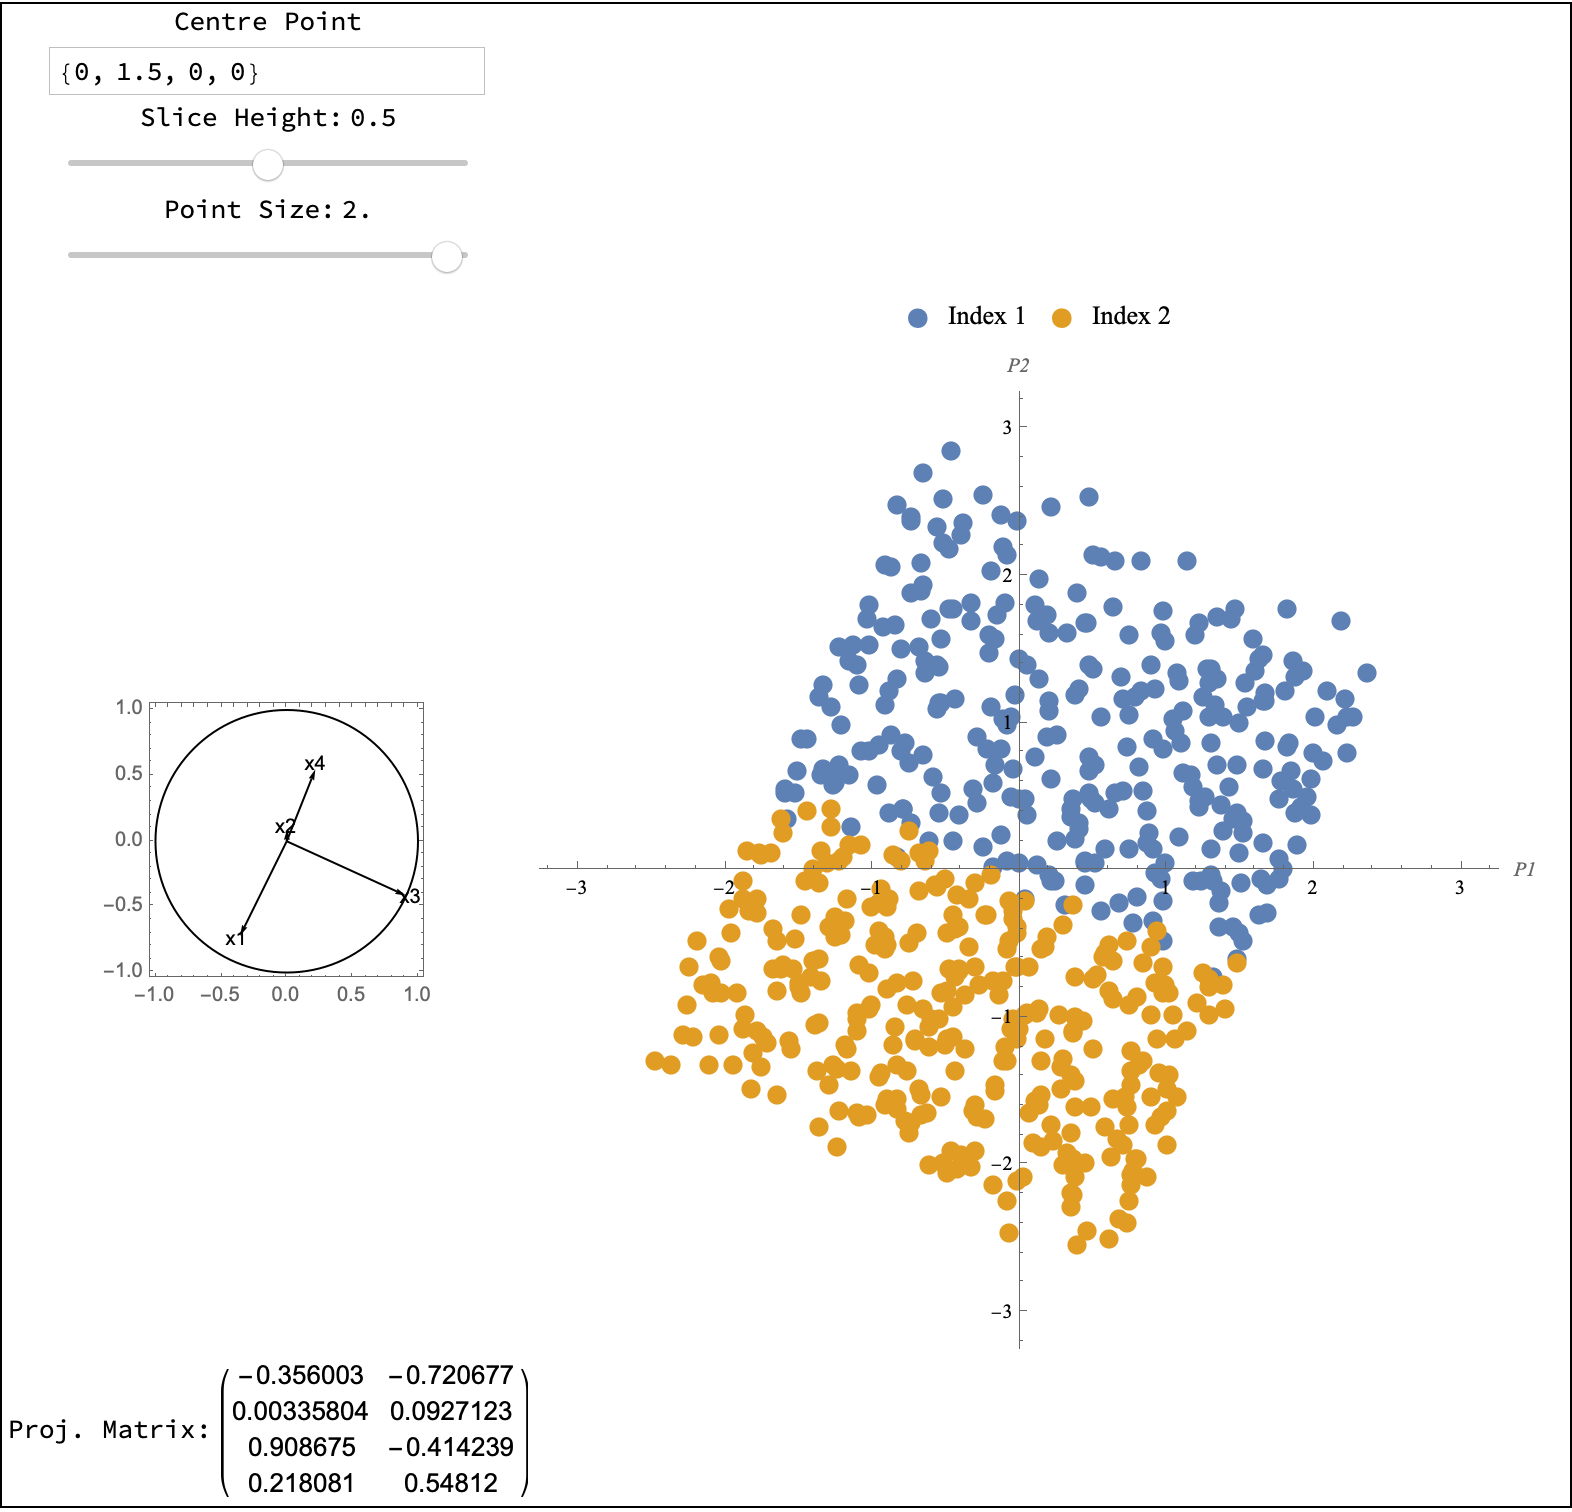
\includegraphics[width=0.32\textwidth]{figures/slice1_p_lda.png}
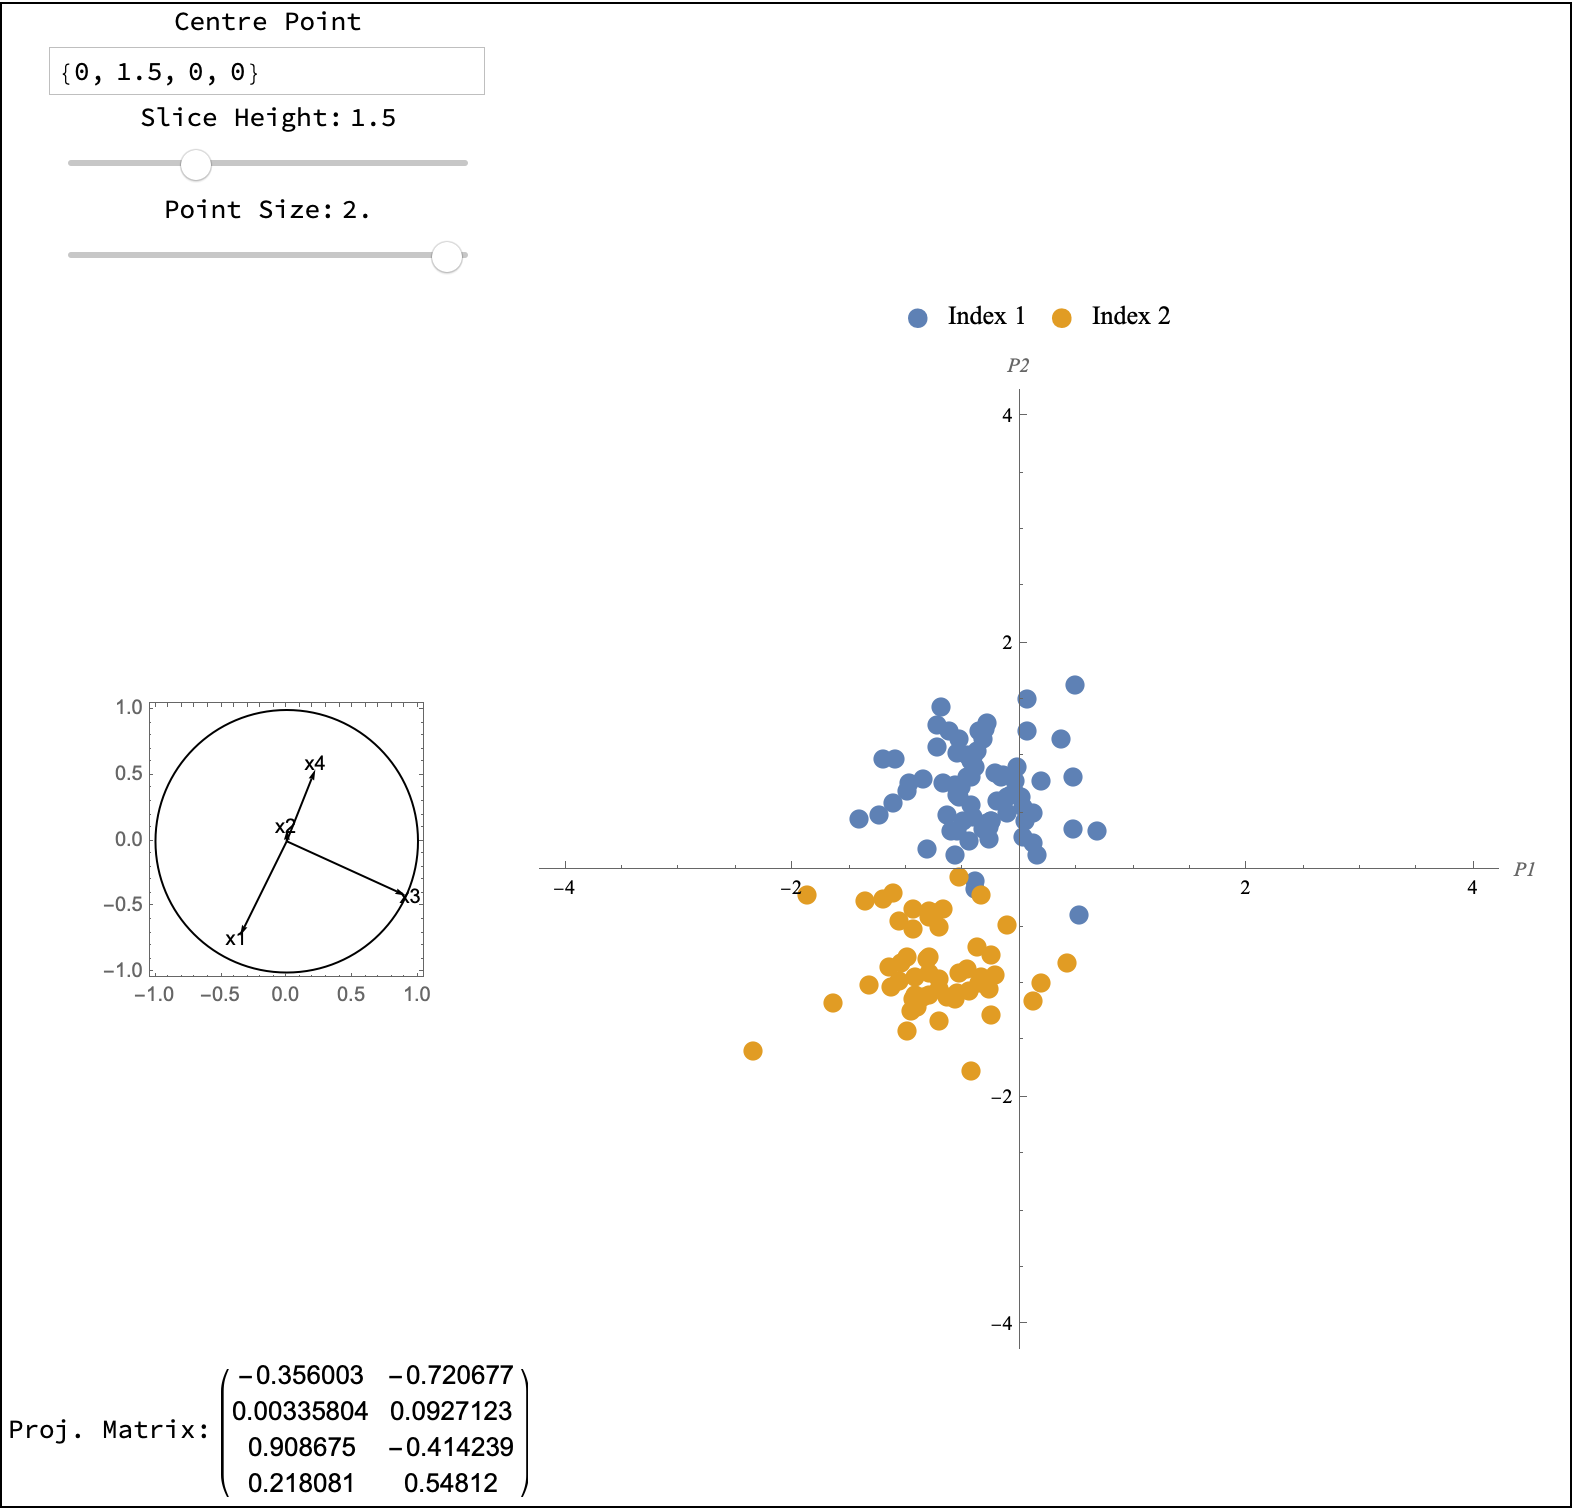
\includegraphics[width=0.32\textwidth]{figures/slice1_p_data.png}}
\caption{...}.
\label{slice1p}
\end{figure*}

A more interesting comparison is found for \(S_1^{-}\), thus the slice
localized towards low values of bill depth, shown in Fig. \ref{slice1m}.
The RF model (left) predicts all three species within this slice, with
an interesting boundary for the third class (green, Gentoo). On the
other hand the LDA model (middle) predominantly predicts the third class
within the slice, this appears to be enforced through the linear
structure of the model. Looking finally at the thick slice through the
data we see that there are primarily observations from this class within
the slice we can conclude that the two models have filled in the
``empty'' space (where we do not have any training observations) in very
different ways and according to what we might expect given the model
structure.

\begin{figure*}[ht]
\centerline{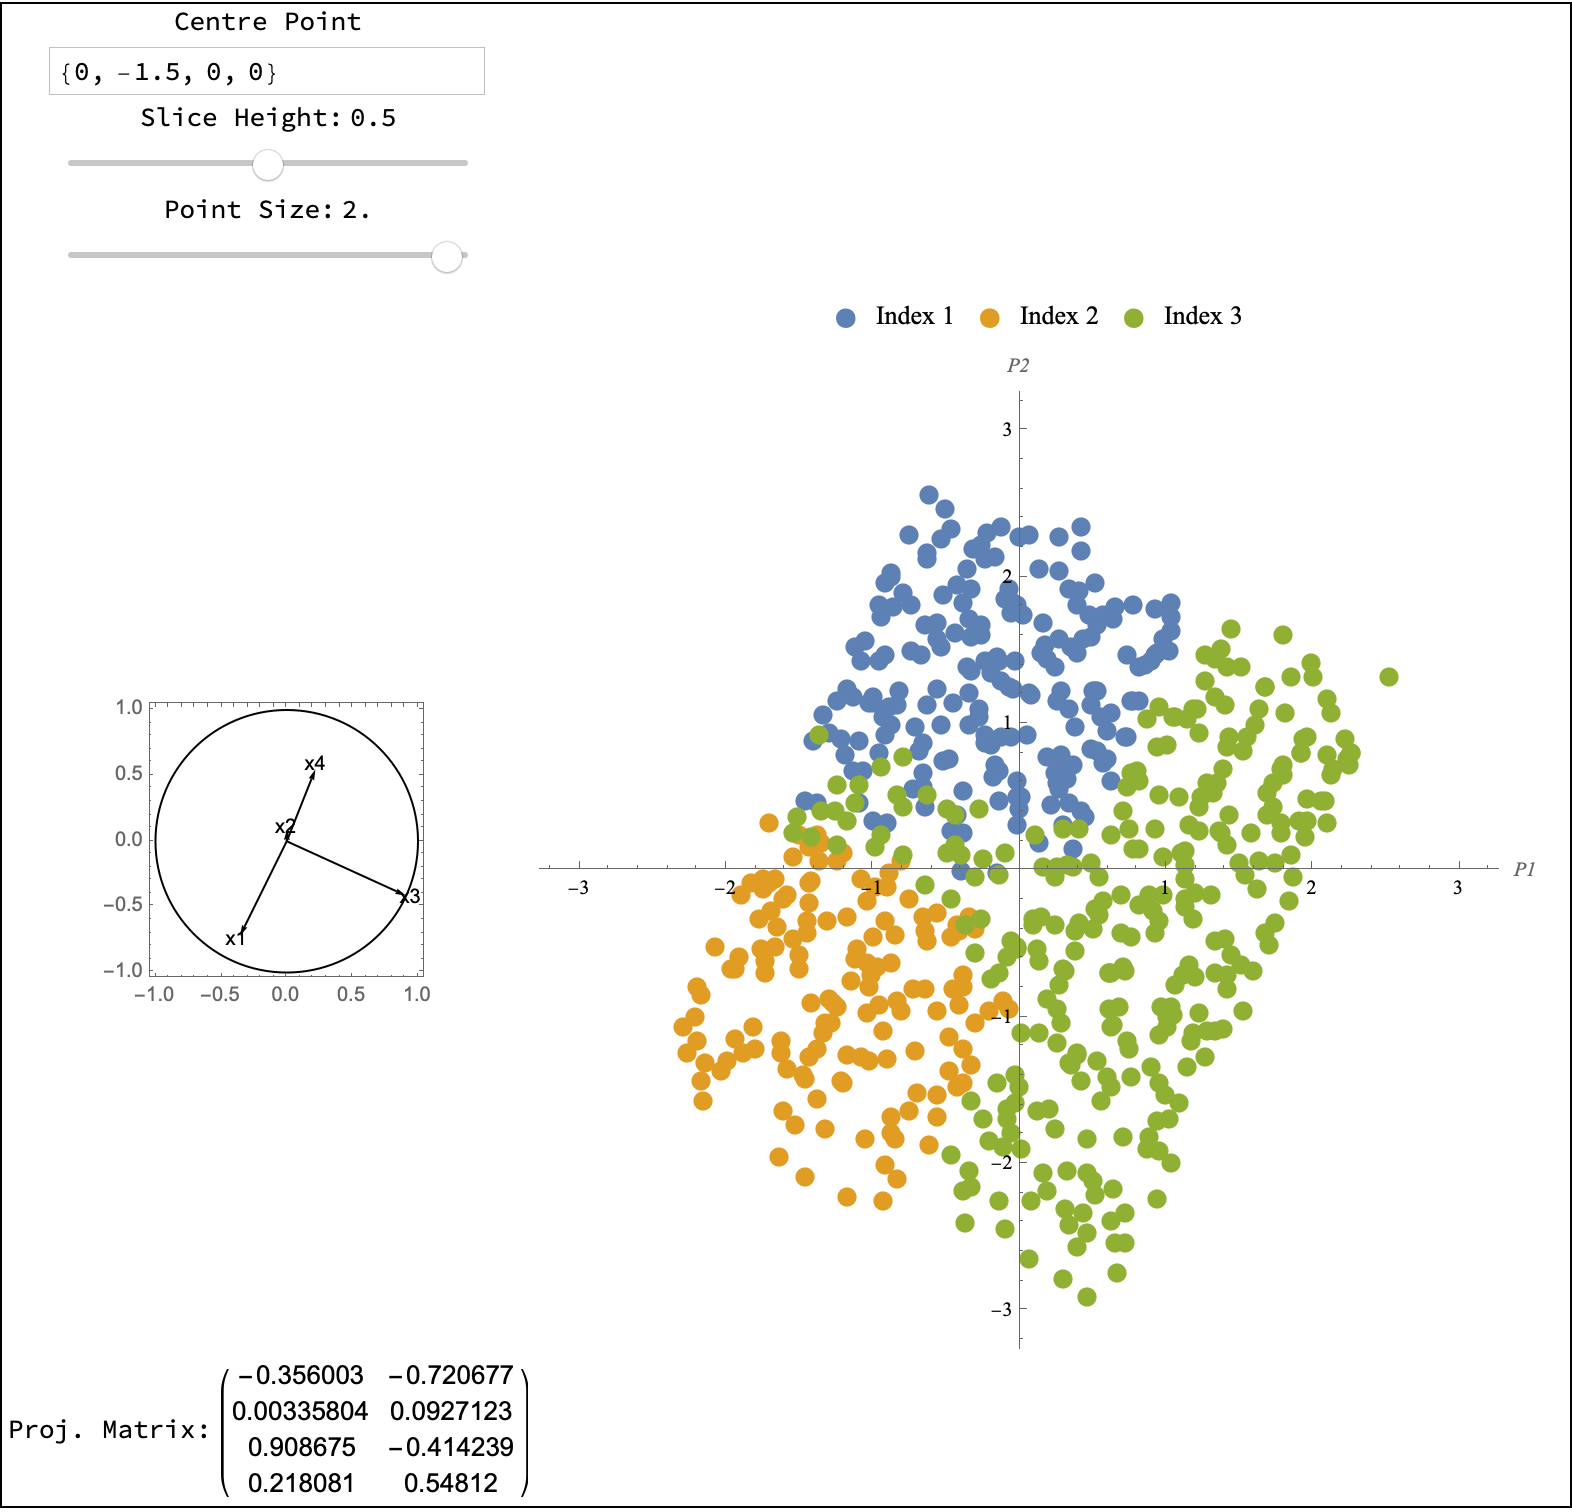
\includegraphics[width=0.32\textwidth]{figures/slice1_m_rf.png}
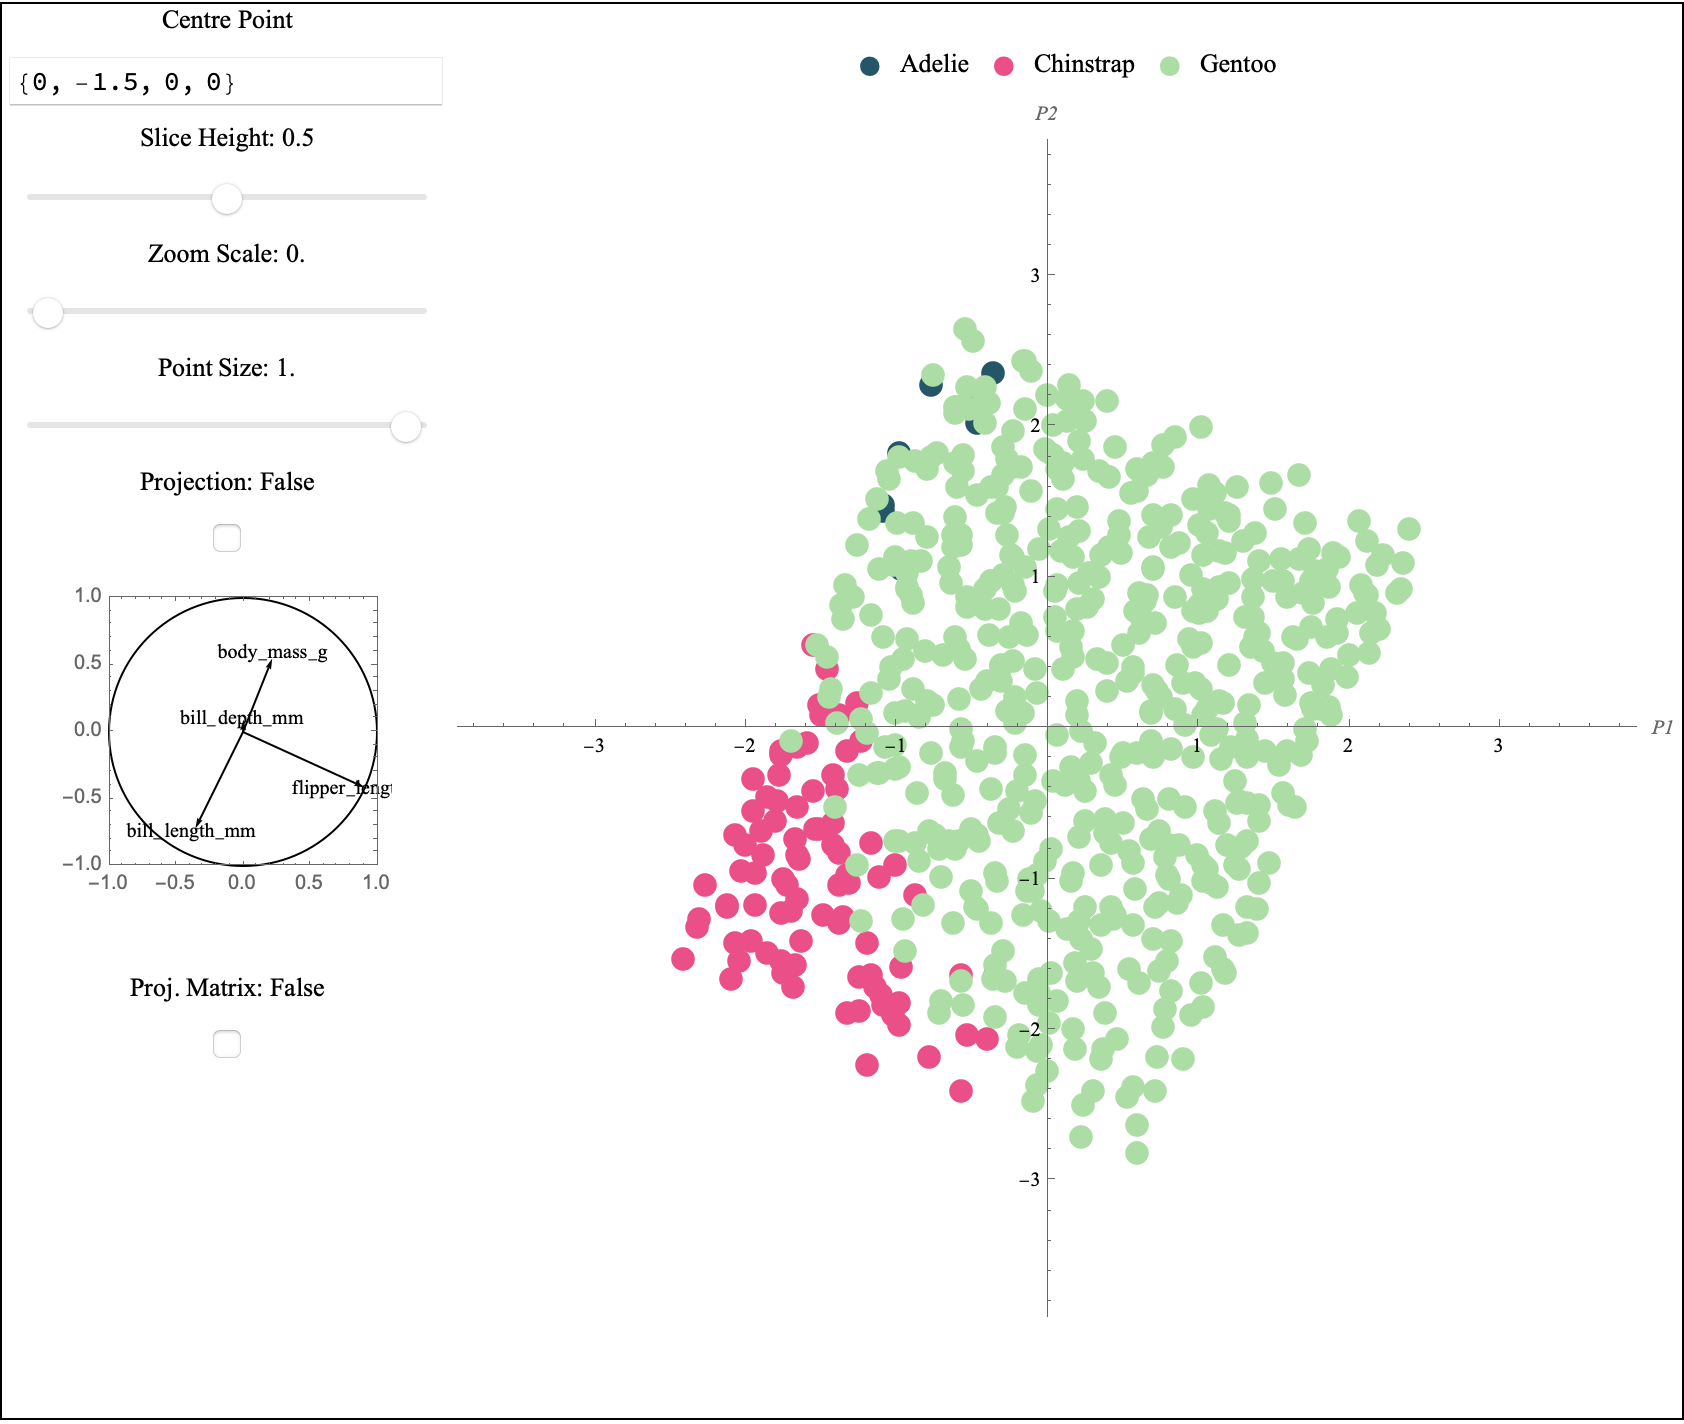
\includegraphics[width=0.32\textwidth]{figures/slice1_m_lda.png}
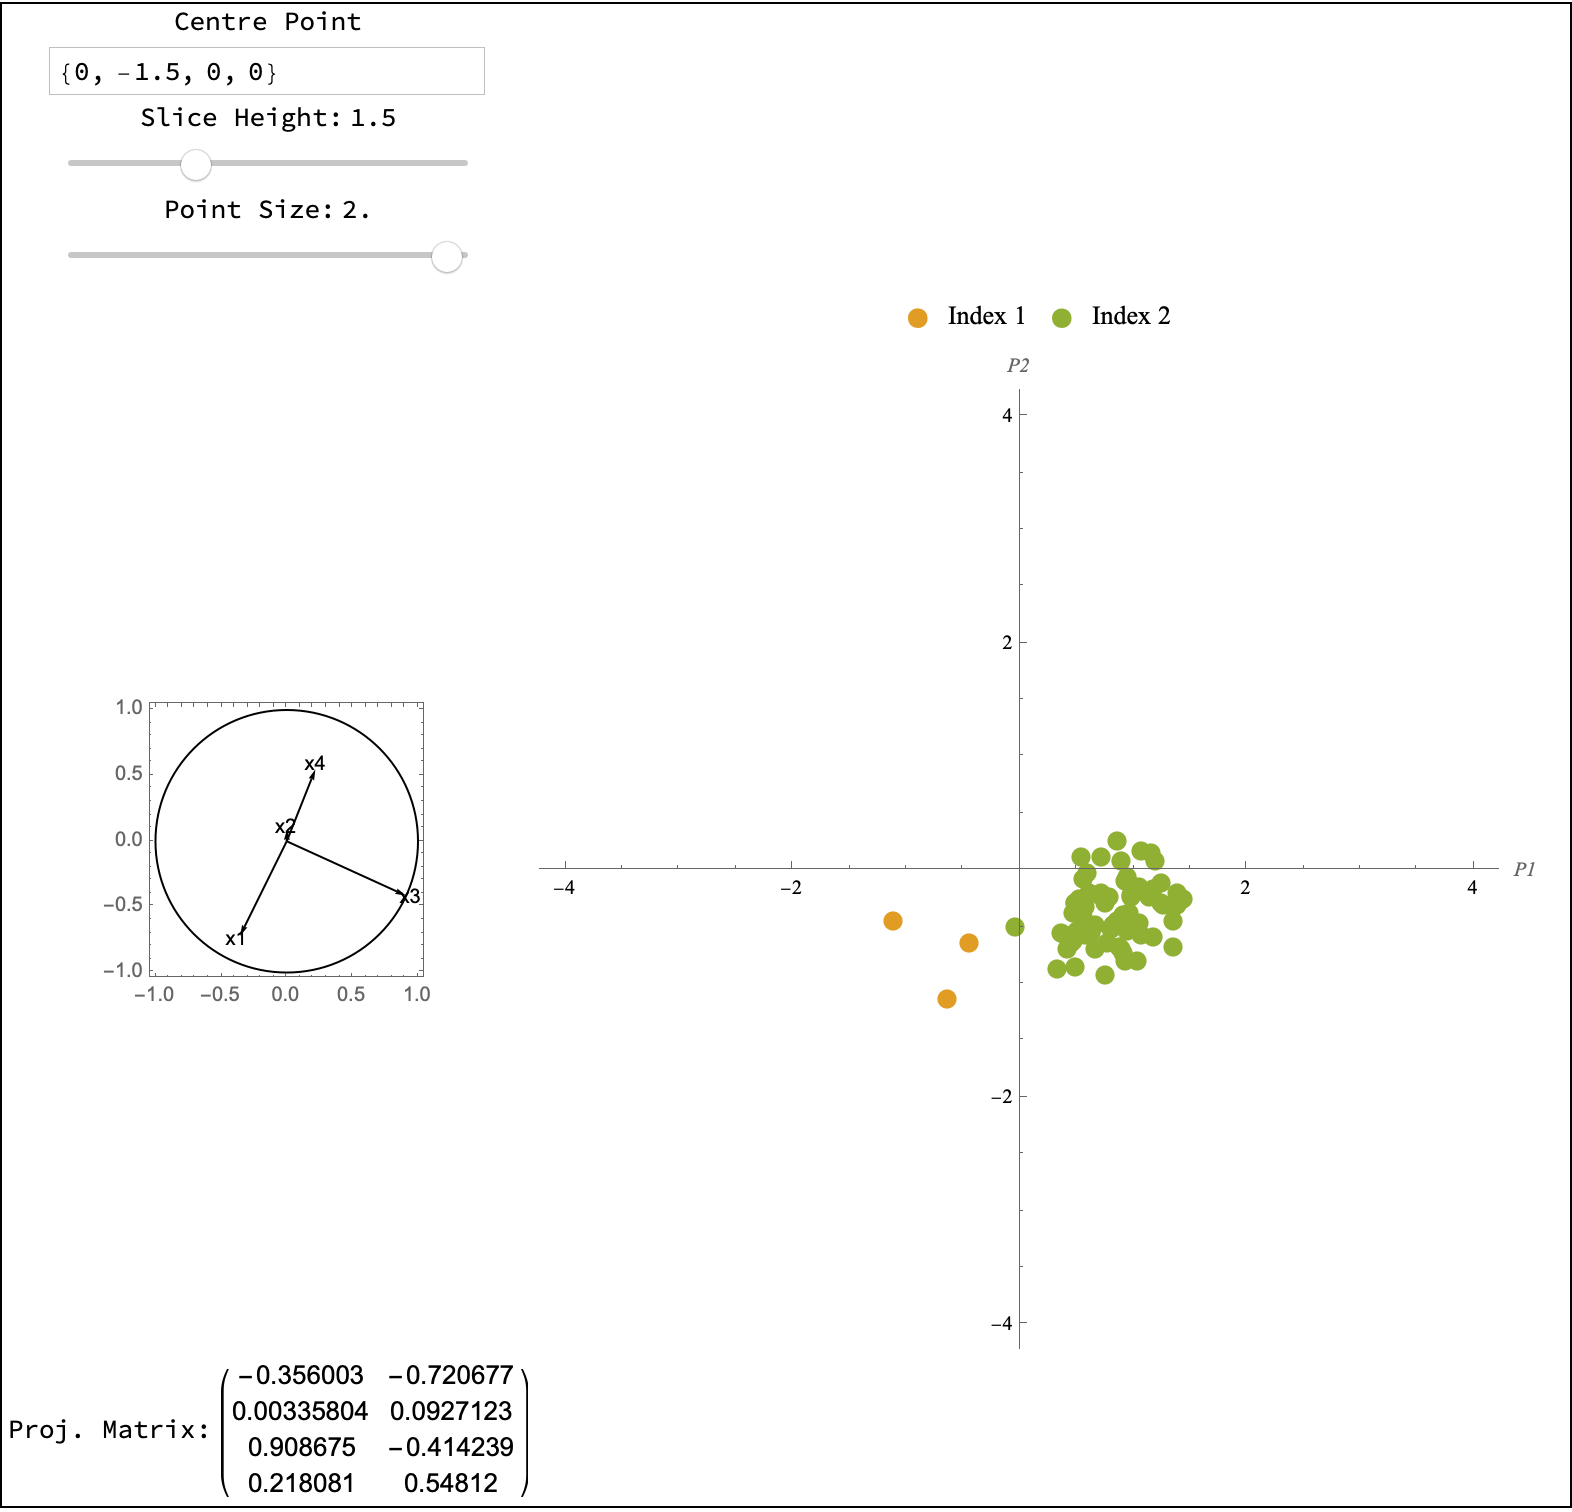
\includegraphics[width=0.32\textwidth]{figures/slice1_m_data.png}}
\caption{...}.
\label{slice1m}
\end{figure*}

Finally it is interesting to compare the slice views to the projection
of the models seen in Fig. \ref{proj1} to better understand how the
boundaries change along the \texttt{bd} direction and where the
differences in the projections come from.

\hypertarget{extension-added-in-the-r-package-tourr}{%
\section{\texorpdfstring{Extension added in the R package
\texttt{tourr}}{Extension added in the R package tourr}}\label{extension-added-in-the-r-package-tourr}}

Explain \texttt{radial\_tour}

\hypertarget{what-would-be-desirable-for-implementations-in-r}{%
\section{What would be desirable for implementations in
R?}\label{what-would-be-desirable-for-implementations-in-r}}

\hypertarget{sec:discussion}{%
\section{Discussion}\label{sec:discussion}}

\hypertarget{acknowledgements}{%
\section*{Acknowledgements}\label{acknowledgements}}
\addcontentsline{toc}{section}{Acknowledgements}

The authors gratefully acknowledge the support of the Australian
Research Council. The paper was written in \texttt{rmarkdown}
\citep{rmarkdown} using \texttt{knitr} \citep{knitr}.

\hypertarget{supplementary-material}{%
\section*{Supplementary material}\label{supplementary-material}}
\addcontentsline{toc}{section}{Supplementary material}

The source material and animated gifs for this paper are available at

\bibliographystyle{tfcad}
\bibliography{biblio.bib}





\end{document}
